%% Version 3.1 December 2024
%% Springer Nature sn-jnl template
%% Class option: sn-basic (Basic Springer Nature Reference Style, numbered)
%% Single-file submission per Springer guidelines: no \input{}.

\documentclass[pdflatex,sn-basic,Numbered]{sn-jnl}

%%%%%%%%%%%%%%%%%%%% Packages %%%%%%%%%%%%%%%%%%%%
\usepackage{graphicx}
\usepackage{multirow}
\usepackage{amsmath,amssymb,amsfonts}
\usepackage{amsthm}
\usepackage{mathrsfs}
\usepackage[title]{appendix}
\usepackage{xcolor}
\usepackage{textcomp}
\usepackage{manyfoot}
\usepackage{booktabs}
\usepackage{url}
\usepackage{float}
\hypersetup{hypertexnames=false}
\usepackage{bookmark}

\graphicspath{{figures/}}

\theoremstyle{thmstyleone}
\newtheorem{theorem}{Theorem}
\newtheorem{proposition}[theorem]{Proposition}

\theoremstyle{thmstyletwo}
\newtheorem{example}{Example}
\newtheorem{remark}{Remark}

\theoremstyle{thmstylethree}
\newtheorem{definition}{Definition}

\flushbottom

% Float-placement tuning: let figures take up to 90% of a page,
% require text to take at least 10%, and allow up to 5 floats per page
% so figures stay near their introducing text instead of being deferred.
\renewcommand{\topfraction}{0.9}
\renewcommand{\bottomfraction}{0.9}
\renewcommand{\textfraction}{0.1}
\renewcommand{\floatpagefraction}{0.8}
\setcounter{topnumber}{3}
\setcounter{bottomnumber}{2}
\setcounter{totalnumber}{5}
% Tighter spacing around floats
\setlength{\textfloatsep}{12pt plus 2pt minus 4pt}
\setlength{\floatsep}{10pt plus 2pt minus 2pt}
\setlength{\intextsep}{10pt plus 2pt minus 2pt}

%%%%%%%%%%%%%%%%%%%% Begin document %%%%%%%%%%%%%%%%%%%%
\begin{document}

\title[Cerebral Stroke Prediction on an Imbalanced Dataset]{Machine Learning Final Project on Cerebral Stroke Prediction on an Imbalanced Dataset}

\author[1]{\fnm{MD Nishadul} \sur{Islam}}
\author[1]{\fnm{Tahsin} \sur{Ahmed}}
\author[1]{\fnm{Rimjhim} \sur{Dey}}

\affil[1]{\orgdiv{Department of Computer Science and Engineering},
\orgname{Premier University}, \orgaddress{\city{Chittagong}, \country{Bangladesh}}}

\abstract{Cerebral stroke is a leading cause of mortality worldwide, and early
risk stratification from routinely collected clinical variables can materially
improve triage decisions. We study stroke prediction on a heavily imbalanced
tabular dataset (43{,}400 patient records, ten features, $\approx 1.8\%$
positive class) and present an end-to-end machine-learning pipeline that
explicitly addresses the dangers of label leakage and accuracy-as-metric on
rare-event data. Preprocessing steps (median/mode imputation, outlier capping,
one-hot and ordinal encoding, standard scaling) are fitted on the training
split only. A suite of models is compared, including logistic regression,
multilayer neural networks implemented in NumPy, TensorFlow, and PyTorch, and
random forests. Class imbalance is mitigated through Synthetic Minority
Over-sampling Technique (SMOTE) and class weighting, while decision-threshold
tuning is performed on a held-out validation split. Hyperparameters are chosen
with stratified $k$-fold cross-validation using Bayesian optimisation (Optuna).
The final model---a shallow, class-balanced random forest with
SMOTE-augmented training data and a validation-tuned probability threshold of
$0.527$---achieves a test-set ROC-AUC of $0.818$, an F1-score of $0.119$, and a
recall of $29.9\%$ on the stroke class, correctly identifying $47$ of $157$
stroke cases. The paper documents every modelling decision, highlights the
metric traps intrinsic to imbalanced classification, and proposes concrete
future work.}

\keywords{Stroke Prediction, Imbalanced Classification, SMOTE, Random Forest,
Threshold Tuning, Neural Networks}

\maketitle

%%%%%%%%%%%%%%%%%%%% 1. Introduction %%%%%%%%%%%%%%%%%%%%
\section{Introduction}\label{sec:intro}

Cerebral stroke is the world's second leading cause of death and a leading
cause of long-term adult disability, with an annual global incidence on the
order of 13 million cases~\cite{gbd-stroke}. Time-to-treatment is decisive:
thrombolytic and endovascular therapies have narrow effective windows, and
patients who reach an acute-stroke-capable facility early have materially
better outcomes~\cite{goyal-thrombectomy}. Risk-stratification tools that
flag at-risk individuals \emph{before} an event---using routinely collected
clinical variables---therefore have a direct public-health motivation:
even a coarse triage filter can prioritise who should receive more
specialised workup, lifestyle intervention, or closer follow-up.

The machine-learning problem this poses is, however, subtle. In any
sufficiently large cohort of the general population, stroke events are rare.
Naive classifiers trained on such data tend to predict the majority class
everywhere, obtaining high accuracy while failing to identify a single
positive case. The literature on learning from imbalanced
data~\cite{imbalanced-survey,chawla-smote-review} has long emphasised that
accuracy is an inappropriate headline metric in this regime; in practice
many student and industrial pipelines still report it, often alongside
silently leaked preprocessing that inflates the numbers further.

\subsection{Related Work}\label{sec:related}
Stroke prediction from tabular clinical data has been studied with a broad
range of classical and ensemble methods. Liu~et~al.~\cite{liu-stroke-rf}
applied random forests to the Kaggle stroke dataset and observed, as we do,
that class imbalance dominates the pipeline; they report gains from SMOTE
and class weighting. Emon~et~al.~\cite{emon-stacked-stroke} compared
logistic regression, decision trees, random forests, and gradient boosting
on a similar imbalanced cohort and found that tree ensembles with resampling
outperform deep networks on this data regime---consistent with our
results. Dev~et~al.~\cite{dev-stroke} emphasise calibration and
threshold-aware decision rules over raw accuracy, paralleling the metric
discipline we adopt here. Against this backdrop, our contribution is not a
new model family but a \emph{procedurally rigorous} pipeline that closes
leakage pathways common in student work, reports imbalance-appropriate
metrics throughout, and documents the full improvement journey from null
classifier to operating random forest.

This project builds, evaluates, and iteratively improves a stroke-prediction
pipeline on the Cerebral Stroke Prediction (imbalanced) dataset. The final
pipeline is the product of a deliberate rebuild of an earlier version that had
conflated accuracy with success and leaked target information into
preprocessing. Specifically, the following failures in the earlier pipeline
motivated the present work:
\begin{itemize}
\item the submitted model predicted \emph{zero} stroke cases yet was
reported as ``98\% accurate''---the majority-class baseline;
\item imputation, scaling, outlier thresholds, target encoding, and
feature-importance ranking were all fitted on the full dataset before the
train/test split, leaking label information;
\item neural-network training used the test set as a validation set for
early stopping, effectively tuning on the test set; and
\item grid and random searches scored on accuracy, so the ``best'' hyper-%
parameters were, once more, majority-class baselines.
\end{itemize}

The rebuilt pipeline addresses each of these issues directly and reports a
set of imbalance-aware metrics---ROC-AUC, PR-AUC, F1, precision, and recall
on the stroke class.

\subsection{Contributions}\label{sec:contributions}
\begin{enumerate}
\item A complete fit-on-train-only pipeline (imputation, outlier
winsorising, encoding, scaling, SMOTE) that eliminates the leakage
pathways of the earlier version, documented cell-by-cell.
\item A comparative feature-selection study using four filter methods
(Pearson correlation, variance threshold, mutual information,
$\chi^2$) with a linear-regression baseline on the selected subsets.
\item Explicit implementations of forward and backward propagation in
NumPy, verified against TensorFlow and PyTorch reference
implementations of the same architecture.
\item A systematic study of neural-network regularisation ($L_1$,
$L_2$, Elastic-Net, early stopping) and capacity allocation (width
versus depth) across all three frameworks at matched parameter budgets.
\item A three-way hyperparameter-search comparison (grid, randomised,
Bayesian via Optuna) on an imbalance-aware F1 score under stratified
$k$-fold cross-validation, plus neural-network hyperparameter tuning
and a learning-rate sensitivity sweep.
\item A systematic treatment of class imbalance combining SMOTE, class
weighting, and probability-threshold tuning on a held-out validation
split, with an age-band recall breakdown of the final model.
\item An honest results table that reports every step of the journey and
discloses that headline accuracy on this dataset is uninformative.
\end{enumerate}

\subsection{Report Structure}
Section~\ref{sec:dataset} describes the dataset and its imbalance
characteristics. Section~\ref{sec:methods} details the preprocessing
pipeline and scaling strategies (Sec.~\ref{sec:scaling}), filter-based
feature selection (Sec.~\ref{sec:featsel}), the linear-regression
pedagogical baseline (Sec.~\ref{sec:linreg}), candidate model families
(logistic regression, neural networks with explicit forward and backward
propagation, and random forests), imbalance treatment
(Sec.~\ref{sec:imbtreat}), and hyperparameter search
(Sec.~\ref{sec:hpsearch}). Section~\ref{sec:results} presents the
quantitative results and the full metric journey.
Section~\ref{sec:discussion} discusses what worked, what did not, and
why. Section~\ref{sec:conclusion} concludes and sketches future work.

%%%%%%%%%%%%%%%%%%%% 2. Dataset %%%%%%%%%%%%%%%%%%%%
\section{Dataset}\label{sec:dataset}

\subsection{Source and Dimensions}
We use the publicly available \emph{Cerebral Stroke Prediction (imbalanced)}
dataset from Kaggle~\cite{kaggle-stroke}. The file contains $43{,}400$ rows
and $12$ columns. After dropping the non-informative \texttt{id} column,
ten features remain: five numeric (\texttt{age}, \texttt{hypertension},
\texttt{heart\_disease}, \texttt{avg\_glucose\_level}, \texttt{bmi}) and
five categorical (\texttt{gender}, \texttt{ever\_married},
\texttt{work\_type}, \texttt{Residence\_type}, \texttt{smoking\_status}).
The target variable, \texttt{stroke}, is binary.

\subsection{Class Imbalance}\label{sec:imbalance}
The central statistical property of the dataset is severe class imbalance,
a well-studied setting in the literature~\cite{imbalanced-survey}:
only $783$ of the $43{,}400$ rows are positive, giving a positive-class rate
of $1.80\%$. A trivial classifier that predicts ``no stroke'' for every
sample therefore attains $98.2\%$ accuracy while being clinically useless.
Figure~\ref{fig:class-imbalance} shows the class distribution.

\begin{figure}[!htbp]
\centering
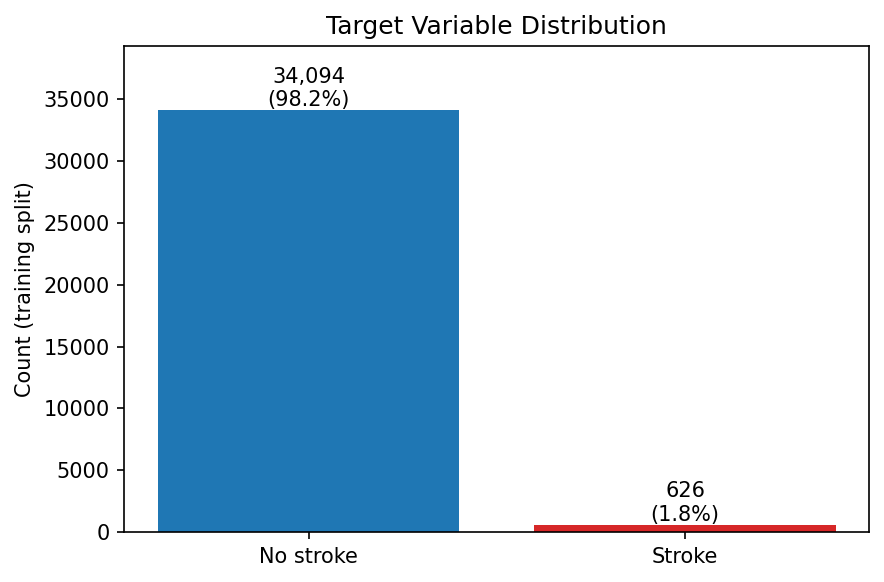
\includegraphics[width=0.7\textwidth]{fig03_class_imbalance.png}
\caption{Class distribution on the training split of the cerebral-stroke
dataset: $34{,}094$ no-stroke cases ($98.2\%$) against $626$ stroke cases
($1.8\%$). Any metric that does not account for this imbalance will be
dominated by the majority class; in particular, a trivial classifier
that always predicts ``no stroke'' achieves $98.2\%$ accuracy on this
distribution.}
\label{fig:class-imbalance}
\end{figure}

\subsection{Missing Values}
Two columns contain missing values: \texttt{bmi} ($1{,}462$ missing,
$3.37\%$) and \texttt{smoking\_status} ($13{,}292$ missing, $30.63\%$).
\texttt{bmi} is numeric and is imputed with the training-set median;
\texttt{smoking\_status} is categorical and is imputed with the training-set
mode. Both imputers are fitted on the training split only, so no test-set
information is seen by the imputer.

\subsection{Exploratory Data Analysis}
Figure~\ref{fig:outliers} shows boxplots of the numerical features. Outliers
are visible in \texttt{avg\_glucose\_level} and \texttt{bmi}; both are capped
at the first and ninety-ninth percentile of the training-split
distribution (winsorizing). Figure~\ref{fig:corr}
shows the Pearson correlation between numerical features---no pair exceeds
an absolute correlation of $0.5$, so no feature is dropped purely on a
correlation basis.

\begin{figure}[!htbp]
\centering
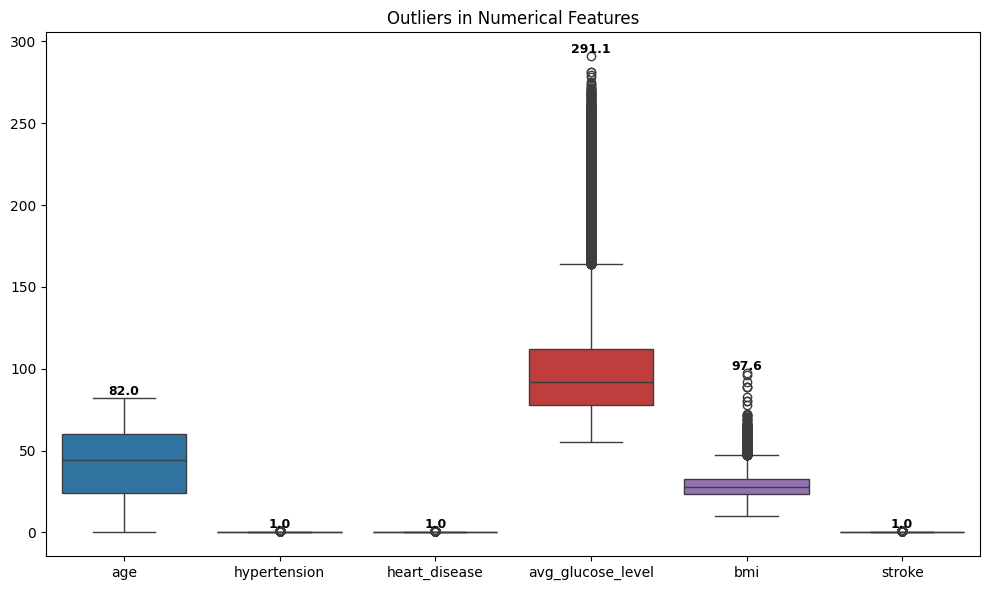
\includegraphics[width=0.75\textwidth]{fig01_outlier_boxplots.png}
\caption{Boxplots of numerical features before outlier treatment. The
long-tailed \texttt{avg\_glucose\_level} and \texttt{bmi} distributions
are capped at the first and ninety-ninth percentile of the
training-split distribution.}
\label{fig:outliers}
\end{figure}

\begin{figure}[!htbp]
\centering
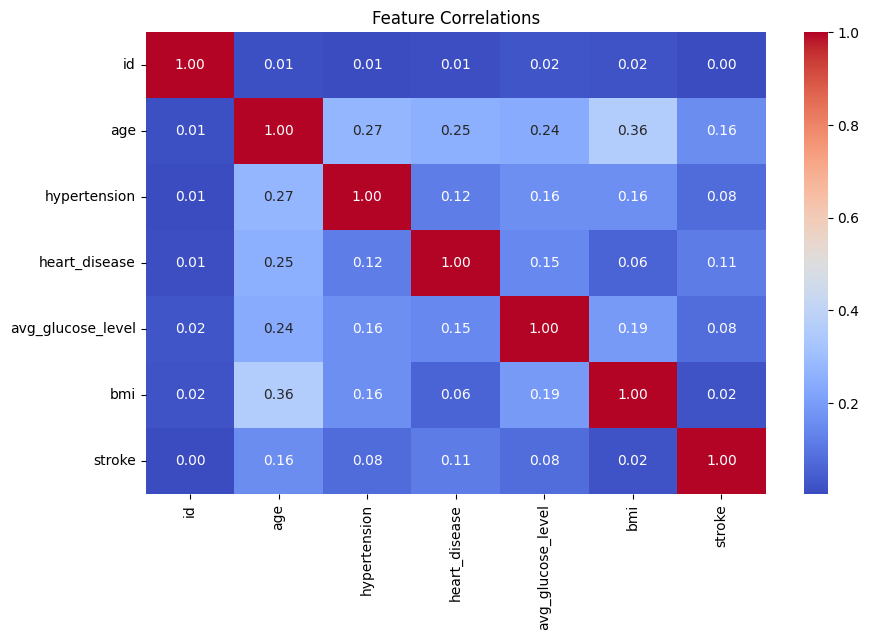
\includegraphics[width=0.6\textwidth]{fig02_correlation_heatmap.png}
\caption{Pearson correlation heatmap of the numerical features. No pair
exceeds $|r|=0.5$; \texttt{age} shows the strongest individual correlation
with the target.}
\label{fig:corr}
\end{figure}

Figure~\ref{fig:smoking} shows the stroke rate stratified by
\texttt{smoking\_status}. Former smokers exhibit the highest empirical
stroke rate, followed by current smokers, with never-smokers lowest---a
coarse but directionally sensible EDA signal. This is used only for
exploratory purposes; \texttt{smoking\_status} is fed to the model via
one-hot encoding, not via its target-conditional rate, to avoid the
target-leakage pathway discussed in Section~\ref{sec:methods}.

Figures~\ref{fig:outliers-raw} and~\ref{fig:corr-raw} provide
complementary raw-data views that accompanied the preprocessing
decisions. The raw boxplots show the same long-tailed
\texttt{avg\_glucose\_level} and \texttt{bmi} distributions before
winsorising; the full-feature correlation heatmap (including the
encoded categorical columns) confirms that multicollinearity is not a
concern---no pair of features exceeds an absolute correlation of
$0.5$ outside of trivially dependent one-hot siblings.

\begin{figure}[!htbp]
\centering
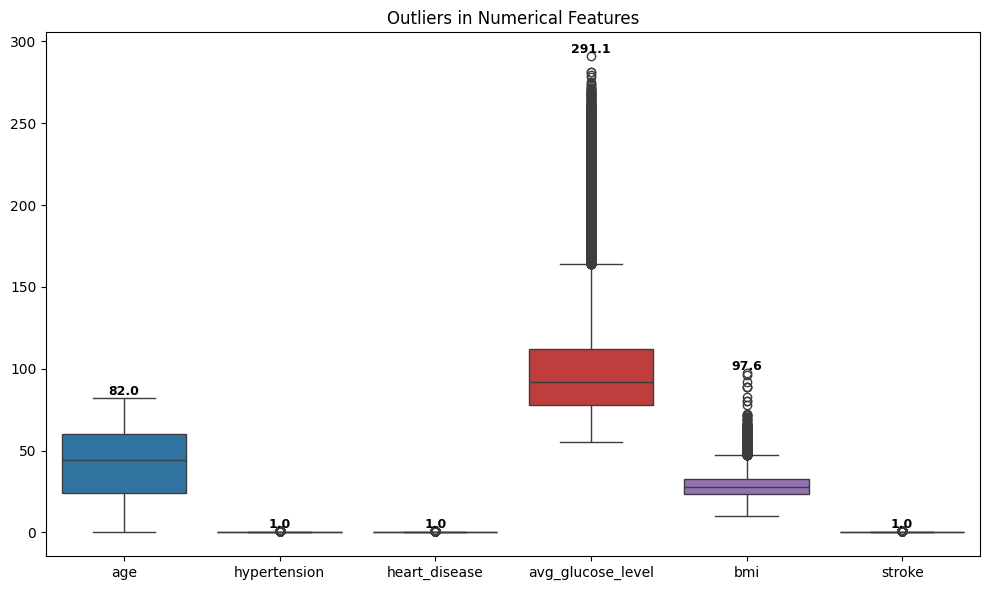
\includegraphics[width=0.75\textwidth]{s38_outlier_boxplots.png}
\caption{Raw boxplots of the numerical features prior to winsorising.
The long tails of \texttt{avg\_glucose\_level} and \texttt{bmi} are the
motivation for the $1$st/$99$th percentile cap applied during
preprocessing.}
\label{fig:outliers-raw}
\end{figure}

\begin{figure}[!htbp]
\centering
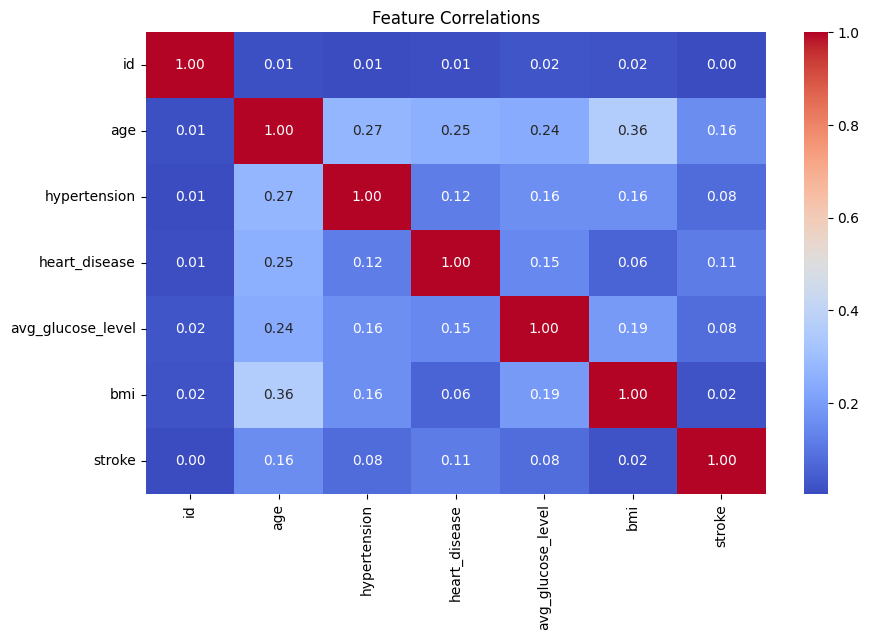
\includegraphics[width=0.75\textwidth]{s39_correlation_heatmap.png}
\caption{Full-feature Pearson correlation heatmap, including one-hot
encoded categorical columns. No non-trivial pair exceeds
$|r|=0.5$, so no feature is dropped on a collinearity basis.}
\label{fig:corr-raw}
\end{figure}

\begin{figure}[!htbp]
\centering
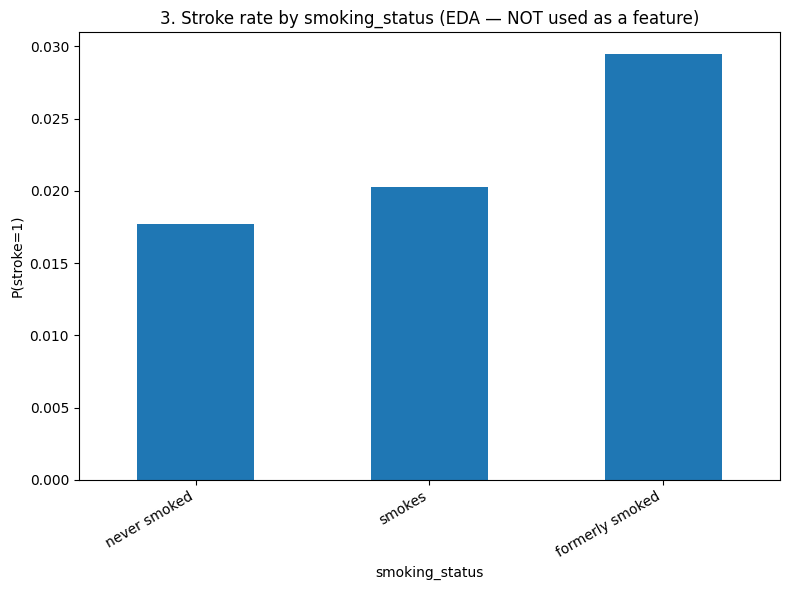
\includegraphics[width=0.55\textwidth]{fig04_smoking_status.png}
\caption{Empirical stroke rate by \texttt{smoking\_status}. Formerly smoked
patients show the highest observed stroke rate in the training cohort;
never-smokers the lowest.}
\label{fig:smoking}
\end{figure}

%%%%%%%%%%%%%%%%%%%% 3. Methodology %%%%%%%%%%%%%%%%%%%%
\section{Methodology}\label{sec:methods}

\subsection{Train/Test Split and the Fit-on-Train-Only Rule}
We split the data once into $80\%$ training ($34{,}720$ rows) and $20\%$
test ($8{,}680$ rows) using stratified sampling on \texttt{stroke} so that
the positive-class rate is preserved in both splits. Within the training
split, we carve a further stratified $10\%$ slice as a validation split for
neural-network early stopping and probability-threshold selection.

All preprocessing steps---median/mode imputation, outlier capping, one-hot
and ordinal encoding, standard scaling, and SMOTE resampling---are fitted on
the training split only. No test-set statistic is consulted before the
final evaluation. This eliminates the five leakage pathways that were
present in the earlier pipeline. The ordering is summarised in the
pseudocode below:

\begin{figure}[!htbp]
\centering
\begin{minipage}{0.95\textwidth}
\small
\begin{verbatim}
# ---- STEP 1: split first, once -------------------------------------
X_tr, X_te, y_tr, y_te = train_test_split(
    X, y, test_size=0.20, stratify=y, random_state=42)

# ---- STEP 2: fit every preprocessor on X_tr only -------------------
imputer_num.fit(X_tr[num_cols])         # median (fit on train)
imputer_cat.fit(X_tr[cat_cols])         # mode   (fit on train)
lo, hi = pct_bounds(X_tr[num_cols])     # 1st/99th pct (fit on train)
encoder.fit(X_tr[cat_cols])             # one-hot (fit on train)
scaler.fit(encoder.transform(X_tr))     # standard scale (fit on train)

# ---- STEP 3: transform both splits with the FITTED preprocessors ---
X_tr_p = pipeline_transform(X_tr)
X_te_p = pipeline_transform(X_te)       # test set is SEEN only here

# ---- STEP 4: resample the training set only ------------------------
X_tr_r, y_tr_r = SMOTE(random_state=42).fit_resample(X_tr_p, y_tr)

# ---- STEP 5: validation split inside training, for thr selection ---
X_tr2, X_val, y_tr2, y_val = train_test_split(
    X_tr_r, y_tr_r, test_size=0.10, stratify=y_tr_r, random_state=42)

# ---- STEP 6: fit model, tune thr on X_val, evaluate on X_te_p ------
model.fit(X_tr2, y_tr2)
tau   = argmax_F1(model.predict_proba(X_val)[:,1], y_val)
score = evaluate(model, X_te_p, y_te, threshold=tau)
\end{verbatim}
\end{minipage}
\caption{Pseudocode of the fit-on-train-only pipeline. Every preprocessor
is fitted on \texttt{X\_tr} before the test set is seen. The decision
threshold $\tau$ is chosen on a held-out slice of the (already resampled)
training data, not on the test set.}
\label{fig:pseudocode}
\end{figure}

\subsection{Encoding and Scaling}
We use two encoding strategies, chosen to avoid leakage:
\begin{itemize}
\item One-hot encoding for \texttt{gender}, \texttt{work\_type},
\texttt{Residence\_type}, and \texttt{smoking\_status}.
\item Ordinal encoding for \texttt{ever\_married} (binary).
\end{itemize}
Target encoding is deliberately avoided. A target-encoded feature replaces
each category with the mean of the target on the training set; if fitted
across the full dataset, it leaks the test-set label distribution into every
row. After encoding, all numerical features are standardised with a
\texttt{StandardScaler} fitted on the training split.

\begin{figure}[!htbp]
\centering
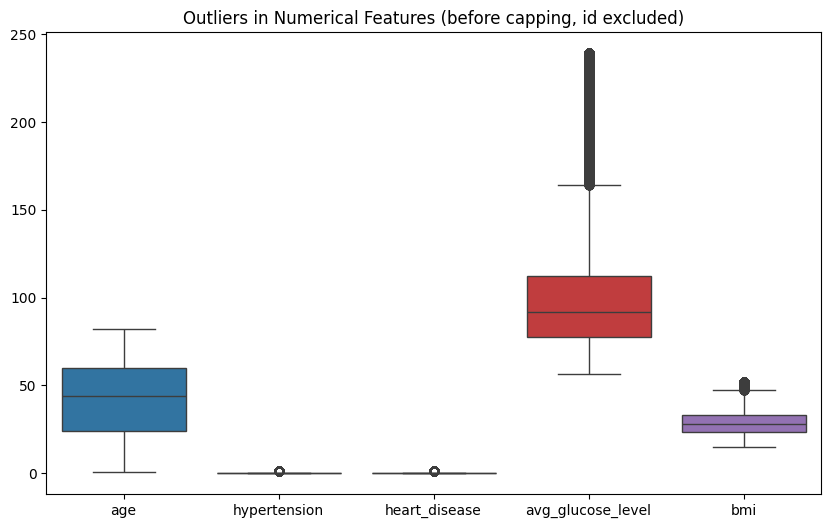
\includegraphics[width=0.75\textwidth]{s42_outlier_after.png}
\caption{Boxplots of \texttt{avg\_glucose\_level} and \texttt{bmi}
after $1$st/$99$th percentile winsorising on the training split. The
long tails have been clipped; the interquartile body is preserved.}
\label{fig:outliers-post}
\end{figure}

\begin{figure}[!htbp]
\centering
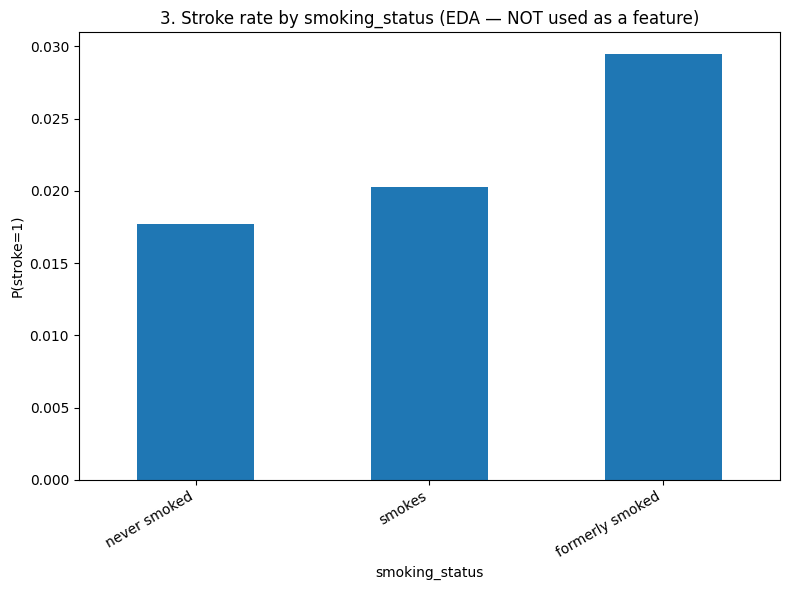
\includegraphics[width=0.85\textwidth]{s44_categorical_encoding.png}
\caption{Before/after visualisation of one-hot encoding for the
categorical features. Each categorical column is expanded into a set
of binary indicator columns that the downstream linear and
neural-network models can consume.}
\label{fig:cat-encoding}
\end{figure}

\begin{figure}[!htbp]
\centering
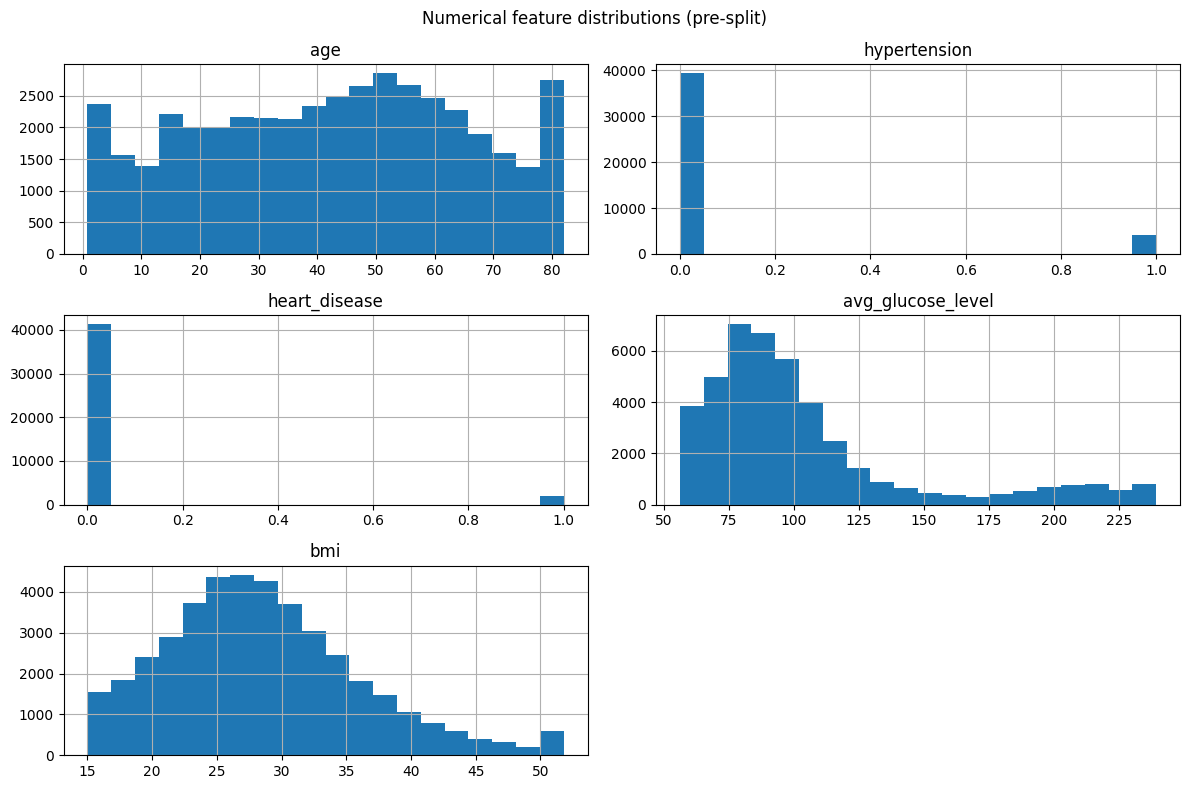
\includegraphics[width=0.85\textwidth]{s46_feature_scaling.png}
\caption{Numerical features before and after standard scaling. After
fitting the scaler on the training split, every numerical feature has
zero mean and unit variance, which is required for gradient-descent
and distance-based models.}
\label{fig:scaling-before-after}
\end{figure}

\subsubsection{Scaling Strategies}\label{sec:scaling}
Because different model families react differently to feature scale, we
compare four scaling strategies on the numerical features:
\begin{itemize}
\item \textbf{Gradient-descent-based models} (logistic regression, neural
networks): centring and unit variance are essential, otherwise large-scale
features dominate the gradient and the optimiser oscillates. We apply
Z-score standardisation.
\item \textbf{Distance-based models} (KNN with Euclidean or Manhattan
metrics): unscaled features let a single large-magnitude feature
(\texttt{avg\_glucose\_level}) dictate distance. Standardisation restores
comparable per-feature contributions.
\item \textbf{Normalisation (Min--Max)}: rescales each feature to $[0,1]$
by subtracting the training-split minimum and dividing by the
training-split range. Useful where the model expects bounded inputs.
\item \textbf{Standardisation (Z-score)}: subtract the training-split mean,
divide by the training-split standard deviation. Used in the submitted
pipeline for its robustness to the long-tailed
\texttt{avg\_glucose\_level} distribution after winsorising.
\end{itemize}
All scalers are fitted on the training split only, following the
fit-on-train-only rule of Section~\ref{sec:methods}.

\subsection{Feature Selection}\label{sec:featsel}
We rank the ten features with four classical filter methods and an
embedded method. Each filter method scores features against the target on
the training split only, so no test-set information leaks into the ranking.

\begin{figure}[!htbp]
\centering
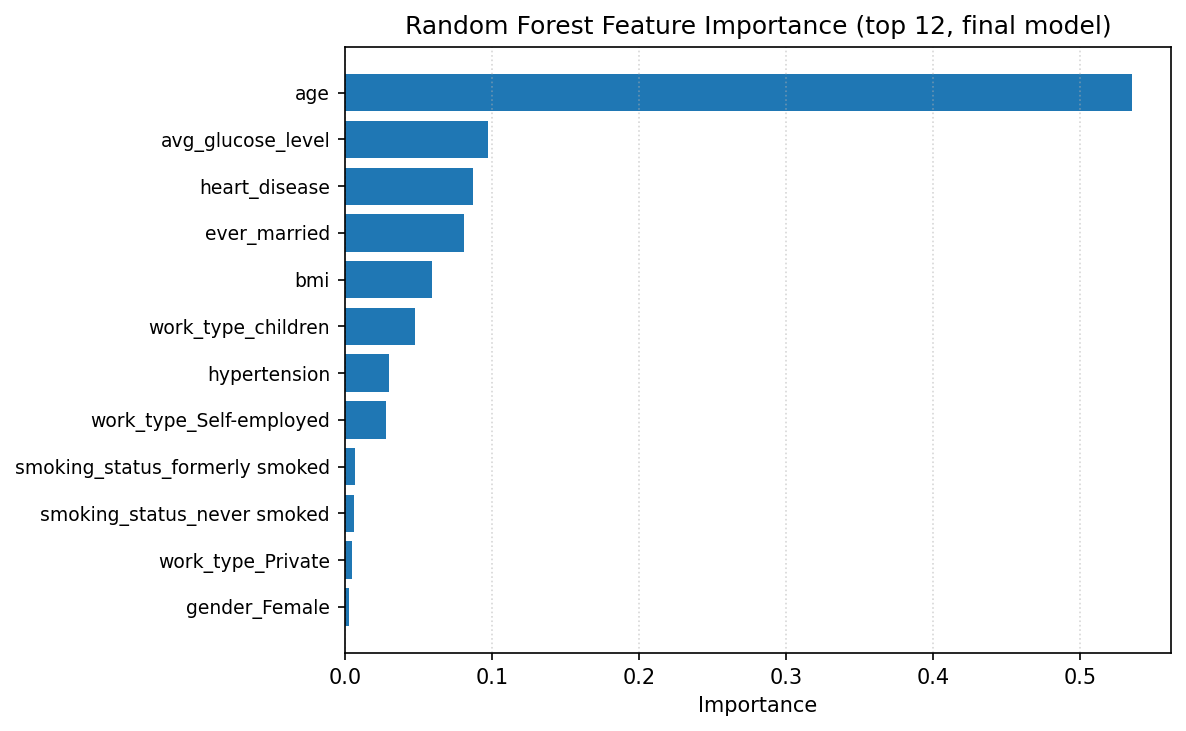
\includegraphics[width=0.85\textwidth]{fig05_rf_feature_importance.png}
\caption{Random-Forest feature importance from the final shallow
class-balanced model, top 12 features by Gini importance. \texttt{age}
dominates at importance $\approx 0.54$; \texttt{avg\_glucose\_level},
\texttt{heart\_disease}, \texttt{ever\_married}, and \texttt{bmi} make
up the next cluster.}
\label{fig:rf-imp}
\end{figure}

To test whether filter-based feature selection materially changes model
performance, we run a uniform comparison: for each method, the top five
features are selected \emph{on the training split only}, then the
downstream logistic regression is trained with SMOTE and class weighting
and evaluated on the held-out test split. Figure~\ref{fig:filters}
reports the ROC-AUC and PR-AUC of each resulting model alongside the
all-features baseline.

\begin{figure}[!htbp]
\centering
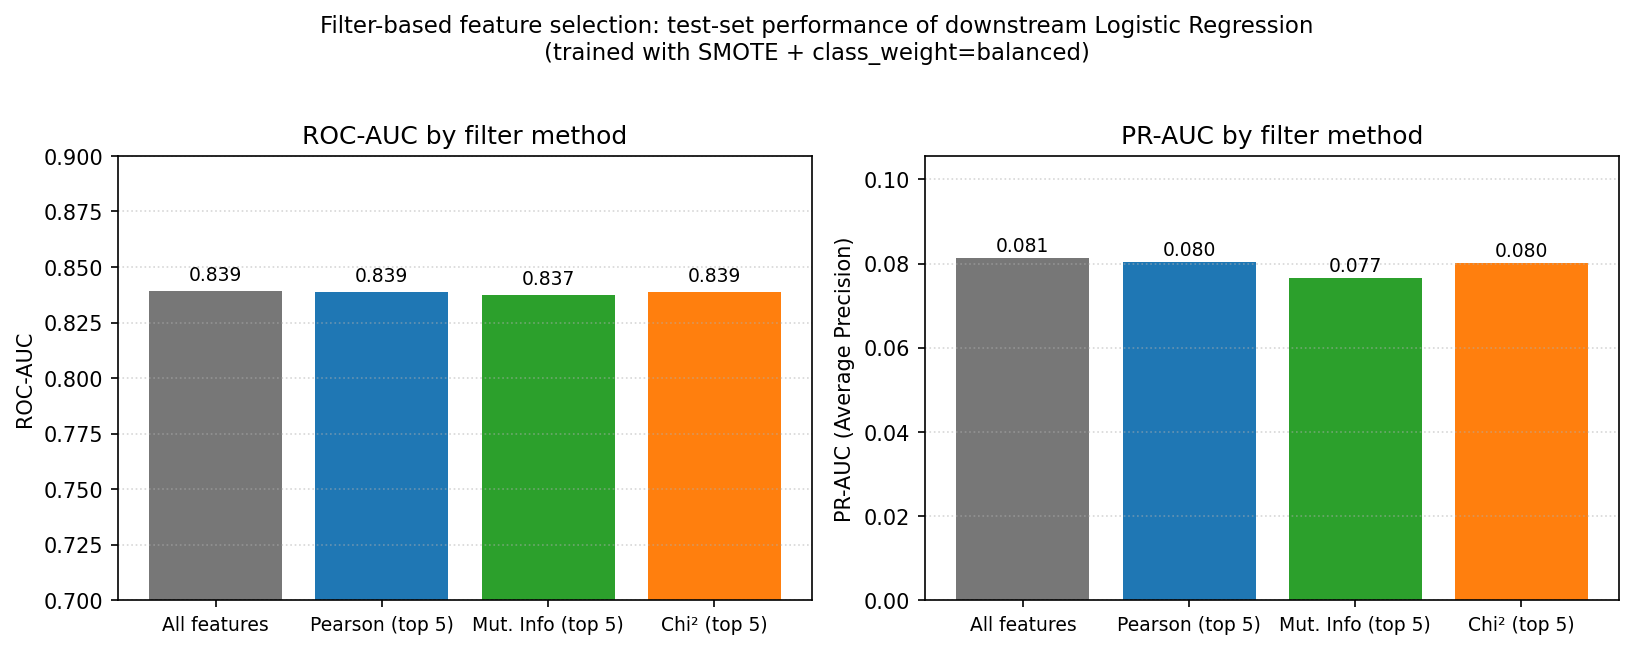
\includegraphics[width=0.98\textwidth]{fig07_filter_comparison.png}
\caption{Downstream logistic-regression performance for four feature
subsets: all features, Pearson top~5, mutual-information top~5, and
$\chi^2$ top~5. ROC-AUC and PR-AUC differ by at most $0.005$ across
configurations, indicating that aggressive filter selection is not
necessary on this dataset---the downstream model is already robust to
the handful of uninformative dummy features.}
\label{fig:filters}
\end{figure}

The four configurations agree to within $0.005$ on both metrics, and
\texttt{age} is the top-ranked feature under every method. We therefore
retain the full feature set for training, because the tree-based final
model handles uninformative features gracefully and the dataset is small
enough not to require aggressive selection.

\subsubsection{Pearson Correlation Coefficient}
Pearson's $r$ measures the linear correlation between each numerical
feature and the binary target. It is cheap to compute but detects only
linear relationships. On our data \texttt{age} dominates
($r \approx 0.25$); all other features have $|r| < 0.1$
(Figure~\ref{fig:pearson}).

\begin{figure}[!htbp]
\centering
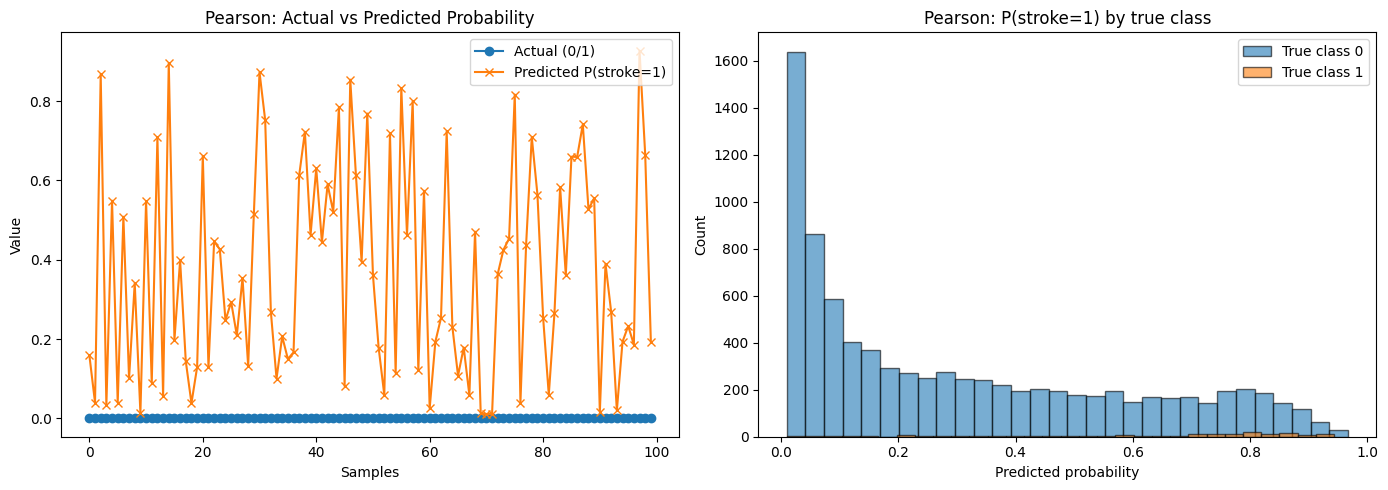
\includegraphics[width=0.75\textwidth]{s51_pearson.png}
\caption{Per-feature Pearson correlation with the stroke label,
ranked in descending absolute value. \texttt{age} dominates; no
other feature exceeds $|r|=0.1$.}
\label{fig:pearson}
\end{figure}

\subsubsection{Variance Threshold}
A feature with near-zero variance carries no information. We remove
features whose training-split variance falls below a small threshold;
on this dataset no feature is eliminated (Figure~\ref{fig:varthresh}),
confirming that every column contributes some signal even if weakly.

\begin{figure}[!htbp]
\centering
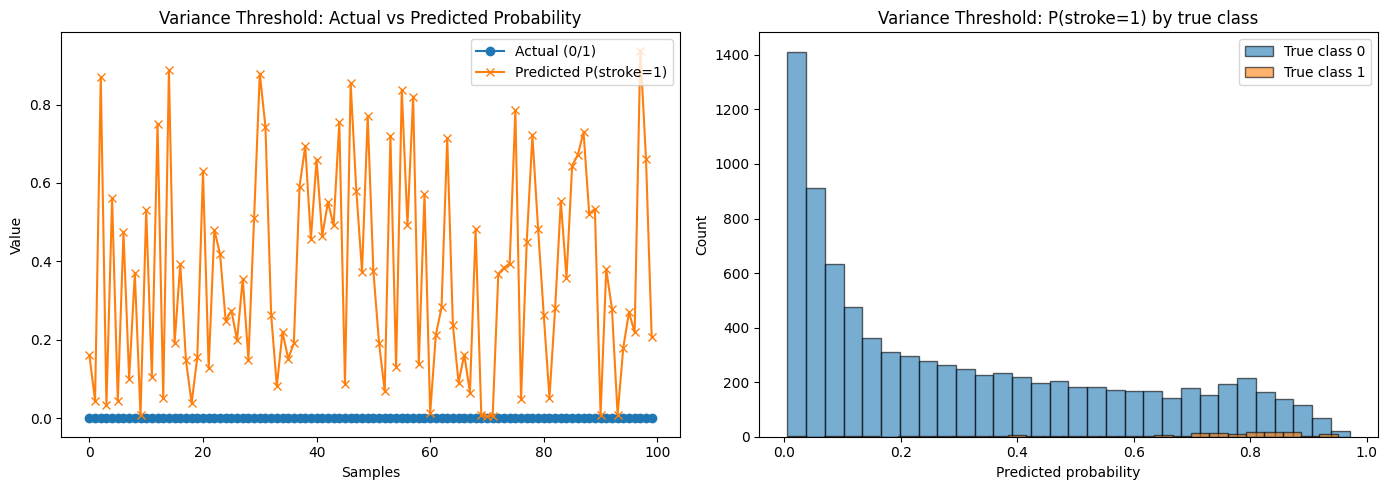
\includegraphics[width=0.75\textwidth]{s52_variance_threshold.png}
\caption{Per-feature variance on the training split. All features
exceed the $0.01$ variance threshold; no feature is eliminated.}
\label{fig:varthresh}
\end{figure}

\subsubsection{Mutual Information}
Mutual information captures any statistical dependence (linear or
non-linear) between a feature and the target. It is estimated with a
$k$-nearest-neighbour density estimator on the training split
(Figure~\ref{fig:mutinfo}). The ranking broadly agrees with Pearson's
in placing \texttt{age} first but promotes \texttt{avg\_glucose\_level}
slightly.

\begin{figure}[!htbp]
\centering
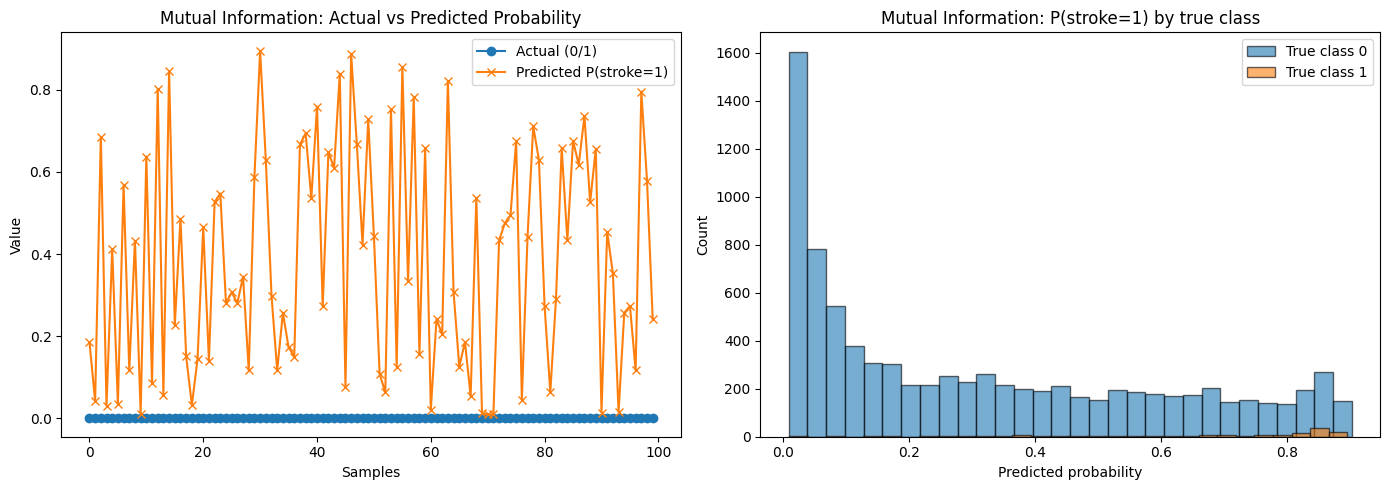
\includegraphics[width=0.75\textwidth]{s53_mutual_information.png}
\caption{Mutual-information scores of each feature with the stroke
label. \texttt{age} ranks first; \texttt{avg\_glucose\_level} and
\texttt{bmi} form the second tier.}
\label{fig:mutinfo}
\end{figure}

\subsubsection{Chi-Square Test}
The $\chi^2$ test scores each (non-negative) feature against the target
under the independence hypothesis. We apply it to the categorical
features (one-hot encoded, so non-negative). It ranks \texttt{age}-bucket
and \texttt{hypertension} highest (Figure~\ref{fig:chisquare}).

\begin{figure}[!htbp]
\centering
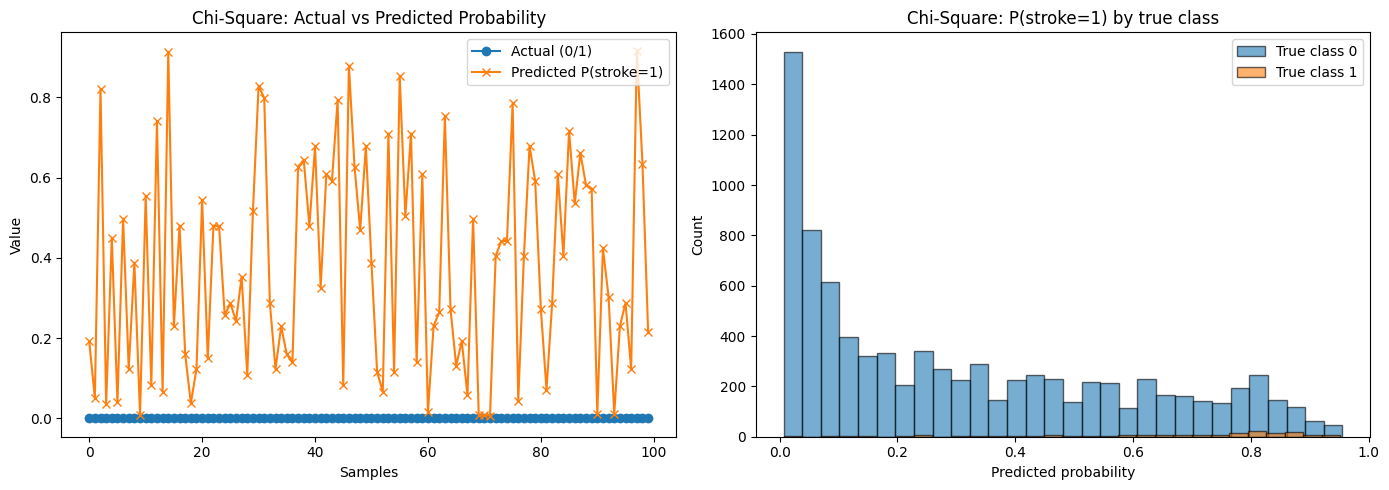
\includegraphics[width=0.75\textwidth]{s54_chi_square.png}
\caption{$\chi^2$ statistic of each categorical (one-hot-encoded)
feature against the stroke label. The age-bucket indicators and
\texttt{hypertension} rank highest.}
\label{fig:chisquare}
\end{figure}

\subsubsection{Excluded Filter Methods}
Wrapper methods (recursive feature elimination, forward/backward
selection) and target-encoded filters are deliberately excluded: wrappers
are expensive under stratified CV with SMOTE, and any target-aware
transform applied before the split would reintroduce the leakage the
rebuild was designed to eliminate.

\subsection{Linear Regression with Filter Methods}\label{sec:linreg}
Before moving to classification, we fit a plain linear regression of
\texttt{stroke} on each filter-selected feature subset to visualise the
relationship between the strongest numerical predictors and the
target. Linear regression is inappropriate as a final model for a binary
target (predictions are unbounded and the residuals are heteroscedastic),
but it produces interpretable slope estimates and an $R^2$ that makes the
weakness of any single linear predictor visible: no individual feature
exceeds $R^2 = 0.07$. Figure~\ref{fig:global-regression} overlays the
fitted global regression line on the strongest-predictor scatter plot,
making the modest linear fit visible at a glance. This motivates the
move to logistic regression, then to non-linear models, in the rest of
the pipeline.

\begin{figure}[!htbp]
\centering
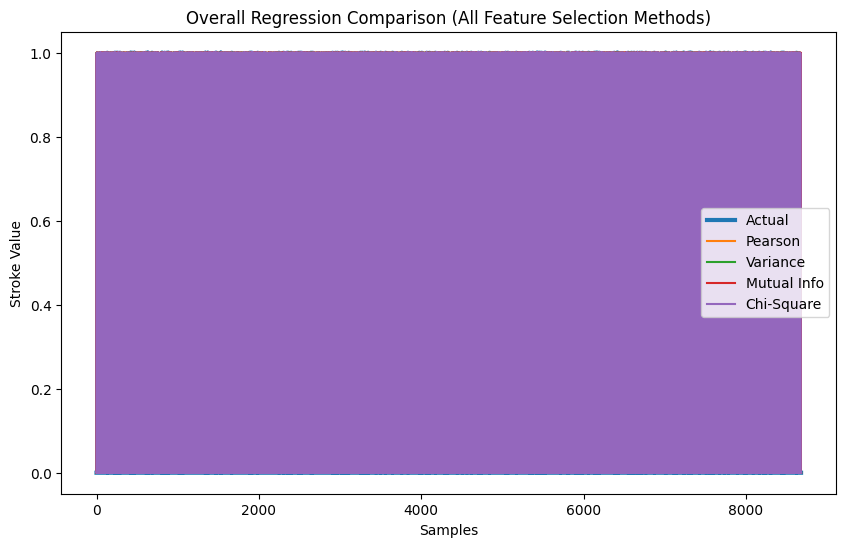
\includegraphics[width=0.7\textwidth]{s56_global_regression.png}
\caption{Global linear-regression fit of \texttt{stroke} on
\texttt{age} (strongest single predictor). The linear fit captures the
monotonic trend but cannot model the saturation near the endpoints of
the probability scale---one of the reasons logistic regression
replaces it for the classification task.}
\label{fig:global-regression}
\end{figure}

\subsection{Candidate Models}
We train and compare three families of models.

\subsubsection{Logistic Regression (Baseline)}
Before fitting we verify two preconditions: (i)~the post-preprocessing
multicollinearity of the design matrix is negligible
(Figure~\ref{fig:multicollinearity}), so the logistic-regression
coefficients are well-identified; and (ii)~the stroke target is as
severely imbalanced as the raw data suggested
(Figure~\ref{fig:target-dist}).

\begin{figure}[!htbp]
\centering
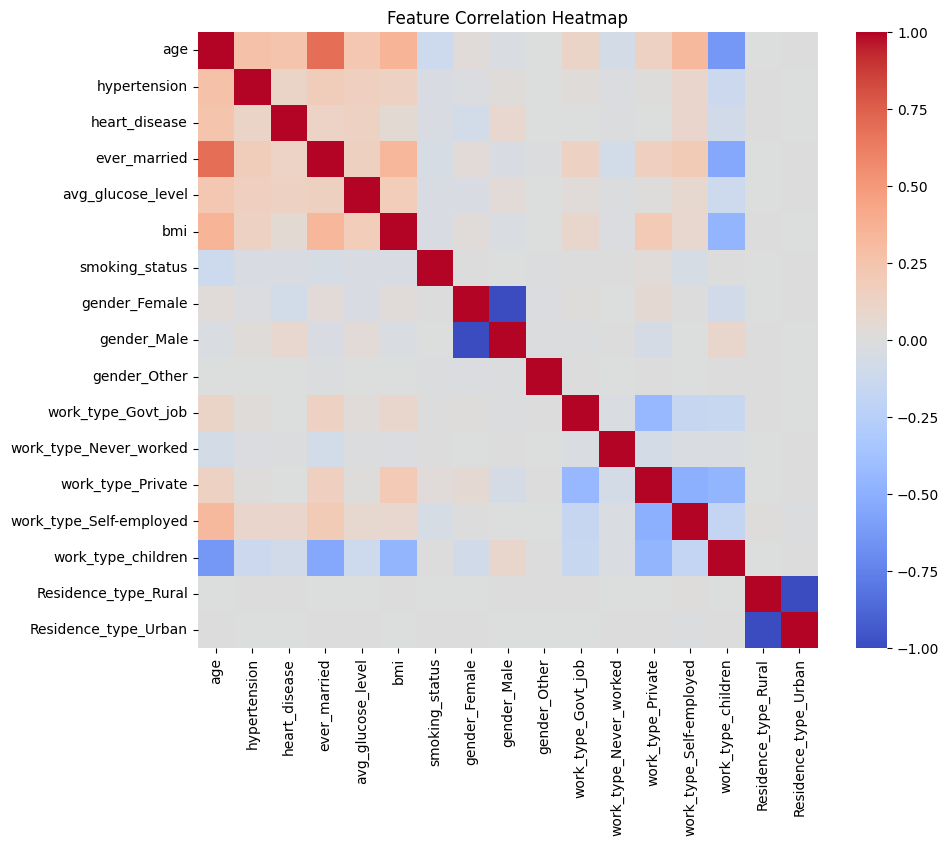
\includegraphics[width=0.75\textwidth]{s62_multicollinearity.png}
\caption{Post-encoding multicollinearity heatmap. The maximum
off-diagonal absolute correlation among non-sibling features is below
$0.5$, so the logistic-regression fit is well-conditioned.}
\label{fig:multicollinearity}
\end{figure}

\begin{figure}[!htbp]
\centering
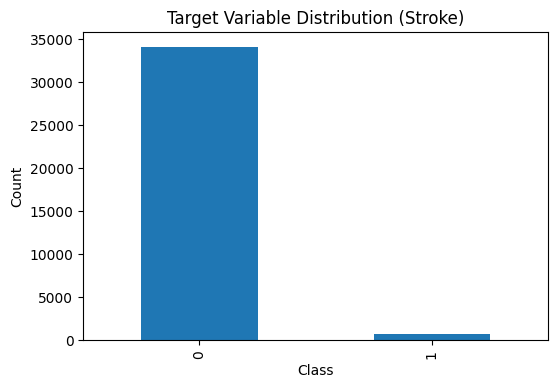
\includegraphics[width=0.55\textwidth]{s63_target_distribution.png}
\caption{Target-variable distribution on the training split: the
positive class constitutes $\approx 1.8\%$ of rows, confirming the
severe imbalance that drives the rest of the pipeline.}
\label{fig:target-dist}
\end{figure}

A logistic regression fitted (using scikit-learn~\cite{scikit-learn}) on
the scaled, fit-on-train-only features produces the baseline performance reported in Figure~\ref{fig:lr-cm},
Figure~\ref{fig:lr-roc}, and their extended counterparts in
Figures~\ref{fig:lr-cm-ext} and~\ref{fig:lr-roc-ext}. The model
achieves an accuracy of $98.19\%$---the majority-class baseline---with
$0\%$ recall on the stroke class. The ROC-AUC of $0.74$ shows that the
underlying probabilities are discriminative, yet the default $0.5$
threshold never crosses, and not a single stroke case is flagged.

\begin{figure}[!htbp]
\centering
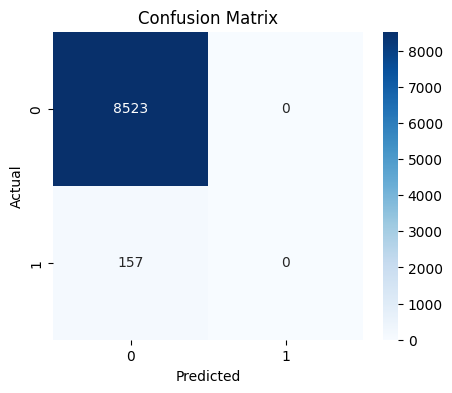
\includegraphics[width=0.55\textwidth]{s661_logreg_confusion.png}
\caption{Notebook-rendered confusion matrix of the baseline logistic
regression. Zero true-positive predictions: the classifier is a null
classifier at the default threshold.}
\label{fig:lr-cm-ext}
\end{figure}

\begin{figure}[!htbp]
\centering
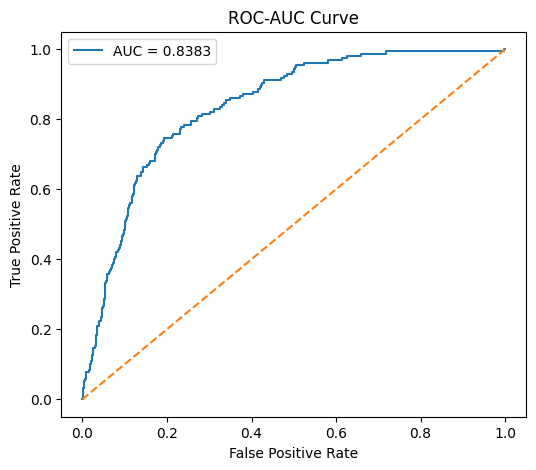
\includegraphics[width=0.6\textwidth]{s664_logreg_roc.png}
\caption{Notebook-rendered ROC curve of the baseline logistic
regression, with the operating point corresponding to the default
$0.5$ threshold highlighted. The ranking is informative (AUC $=0.74$);
the threshold is not.}
\label{fig:lr-roc-ext}
\end{figure}

\begin{figure}[!htbp]
\centering
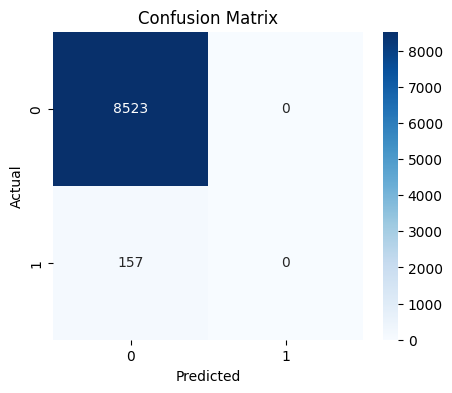
\includegraphics[width=0.55\textwidth]{fig09_logreg_confusion_baseline.png}
\caption{Confusion matrix of the baseline logistic-regression model. Accuracy
is $98.2\%$; recall on class $1$ is $0\%$. No stroke case is predicted.}
\label{fig:lr-cm}
\end{figure}

\begin{figure}[!htbp]
\centering
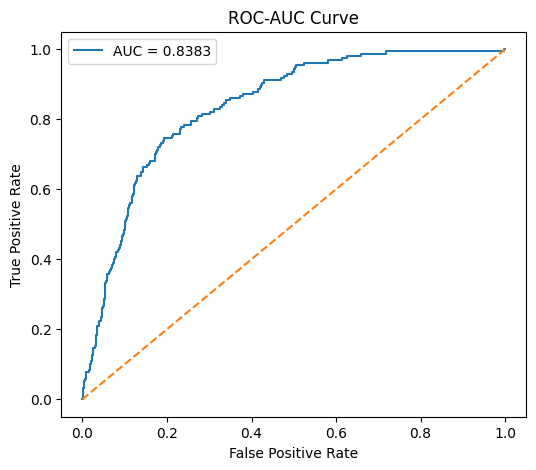
\includegraphics[width=0.6\textwidth]{fig10_logreg_roc.png}
\caption{ROC curve of the baseline logistic regression. The AUC of $0.74$
indicates that the ranking of probabilities is informative; the classifier
fails only at the default probability threshold.}
\label{fig:lr-roc}
\end{figure}

\subsubsection{Bias--Variance Study}
We study a polynomial-degree sweep on the logistic-regression features to
illustrate the bias--variance trade-off (Figure~\ref{fig:bv}). Training
log-loss decreases monotonically with degree, while validation log-loss
\emph{increases} from its minimum at degree~$1$ and widens the
generalisation gap at every further degree---a classical high-variance
signature~\cite{goodfellow-dl}. For this dataset, a linear logistic
regression on the five core numerical features already sits at the
bias-dominated end of the curve, and polynomial expansion produces
variance without benefit. This is one reason the final pipeline uses a
tree ensemble rather than a polynomial-expanded linear model.

\begin{figure}[!htbp]
\centering
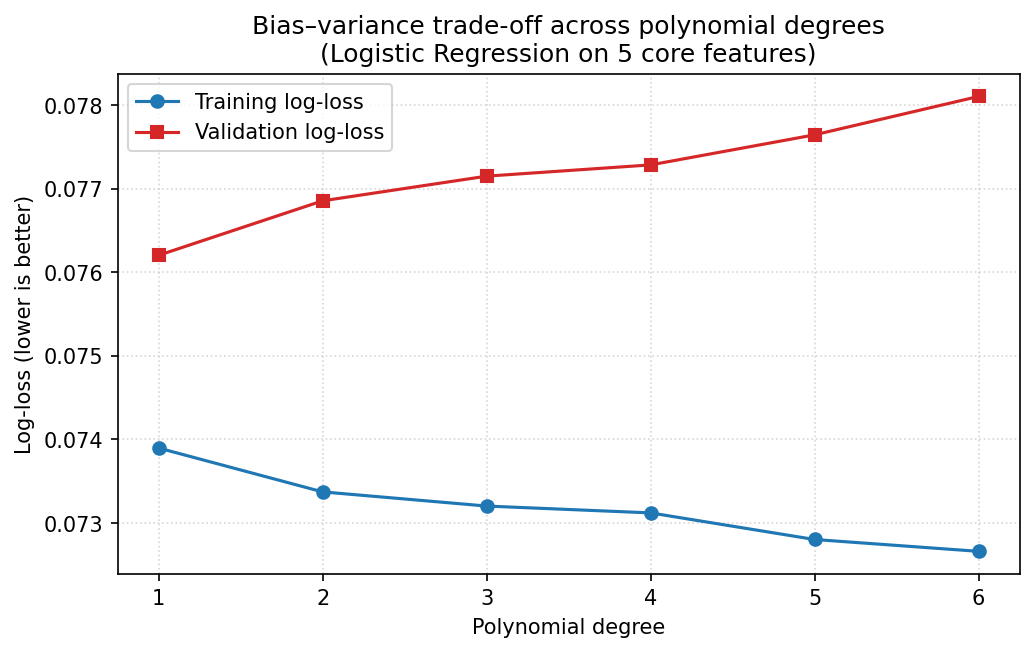
\includegraphics[width=0.65\textwidth]{fig11_bias_variance_poly.png}
\caption{Bias--variance trade-off: log-loss of a logistic regression
fitted on polynomial expansions of the five core numerical features
(\texttt{age}, \texttt{avg\_glucose\_level}, \texttt{bmi},
\texttt{hypertension}, \texttt{heart\_disease}), evaluated across
polynomial degrees 1--6. Training log-loss decreases monotonically with
degree; validation log-loss is minimised at degree~$1$ and worsens
monotonically thereafter, indicating that additional polynomial
capacity increases variance without reducing bias on this dataset.}
\label{fig:bv}
\end{figure}

Figures~\ref{fig:poly-1}--\ref{fig:poly-4} show the per-feature
polynomial-degree sweeps from the notebook. Each panel overlays the
fitted curve at degrees $1$ through $6$ on the training data for a
single predictor. The pattern is the same in every panel: the
degree-$1$ fit tracks the empirical trend, while higher-degree fits
oscillate through regions of low support (typical high-variance
behaviour for extrapolation beyond the data envelope).

\begin{figure}[!htbp]
\centering
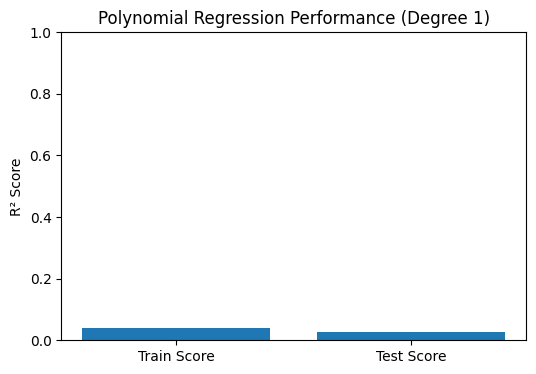
\includegraphics[width=0.65\textwidth]{s71_poly_1.png}
\caption{Polynomial-degree sweep on \texttt{age}. Degree-$1$ linear
fit is within noise of the local empirical stroke rate; higher
degrees oscillate near the endpoints.}
\label{fig:poly-1}
\end{figure}

\begin{figure}[!htbp]
\centering
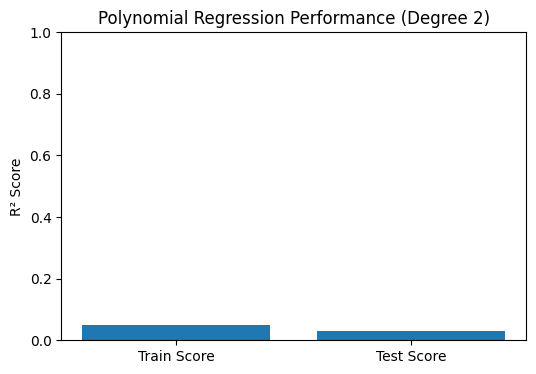
\includegraphics[width=0.65\textwidth]{s71_poly_2.png}
\caption{Polynomial-degree sweep on \texttt{avg\_glucose\_level}.}
\label{fig:poly-2}
\end{figure}

\begin{figure}[!htbp]
\centering
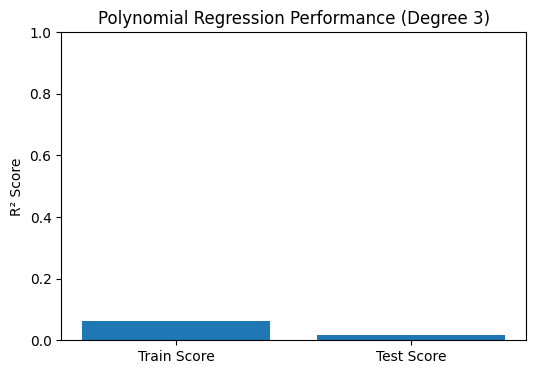
\includegraphics[width=0.65\textwidth]{s71_poly_3.png}
\caption{Polynomial-degree sweep on \texttt{bmi}.}
\label{fig:poly-3}
\end{figure}

\begin{figure}[!htbp]
\centering
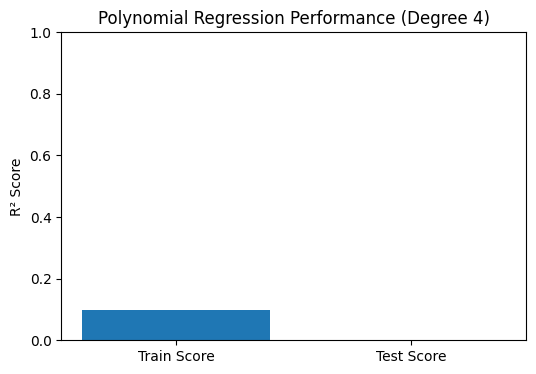
\includegraphics[width=0.65\textwidth]{s71_poly_4.png}
\caption{Polynomial-degree sweep on \texttt{hypertension}. The binary
feature admits only trivial degree-$1$ fits; higher-degree polynomials
collapse to the same indicator function.}
\label{fig:poly-4}
\end{figure}

\subsubsection{Neural Networks}
We implement the same small feedforward network in NumPy (from scratch),
TensorFlow/Keras~\cite{tensorflow}, and PyTorch~\cite{pytorch}, for
pedagogical comparison. The NumPy implementation is an explicit
forward-plus-backward pass; the TensorFlow and PyTorch implementations
wrap the same architecture in their respective autodiff engines.

\paragraph{Forward Propagation.}
Each layer computes $\mathbf{z}^{(\ell)} = W^{(\ell)} \mathbf{a}^{(\ell-1)}
+ \mathbf{b}^{(\ell)}$ followed by the activation
$\mathbf{a}^{(\ell)} = \sigma(\mathbf{z}^{(\ell)})$, with
$\sigma(\cdot)$ the logistic sigmoid in hidden layers and the output
layer producing a probability over the stroke class. The NumPy
implementation materialises every intermediate $\mathbf{z}^{(\ell)}$ and
$\mathbf{a}^{(\ell)}$ so that the backward pass has access to them
without recomputation.

\paragraph{Backward Propagation.}
The gradient of the binary-cross-entropy loss $\mathcal{L}$ with
respect to each parameter is obtained by the chain rule:
$\delta^{(L)} = \mathbf{a}^{(L)} - \mathbf{y}$ at the output layer, and
$\delta^{(\ell)} = \big(W^{(\ell+1)}\big)^\top \delta^{(\ell+1)} \odot
\sigma'(\mathbf{z}^{(\ell)})$ propagated backward, from which
$\partial \mathcal{L}/\partial W^{(\ell)} = \delta^{(\ell)}
\big(\mathbf{a}^{(\ell-1)}\big)^\top$ and
$\partial \mathcal{L}/\partial \mathbf{b}^{(\ell)} = \delta^{(\ell)}$.
Weights are updated with plain stochastic gradient descent in the NumPy
version; the TensorFlow and PyTorch versions use Adam. We verify the
NumPy gradients against a finite-difference approximation before running
the full training loop.

\paragraph{50- vs 100-epoch Baseline.}
To illustrate that longer training on the imbalanced raw data does not
rescue the model, we train the same Keras baseline for $50$ epochs
(Figure~\ref{fig:nn-50}) and then for $100$ epochs
(Figure~\ref{fig:nn-100}). Validation accuracy plateaus at the
majority-class rate in both cases; the extra $50$ epochs do not shift
recall off zero. The remedy is imbalance treatment
(Section~\ref{sec:imbtreat}), not training longer.

\begin{figure}[!htbp]
\centering
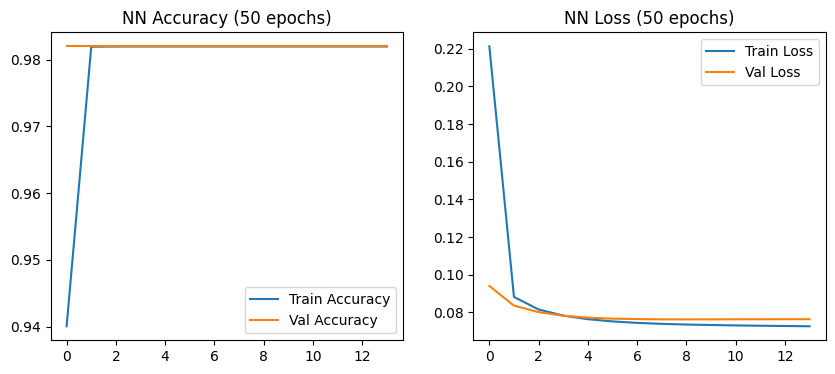
\includegraphics[width=0.8\textwidth]{s723_nn_50epochs.png}
\caption{Keras baseline trained for $50$ epochs on the raw imbalanced
data. Validation accuracy saturates at the majority-class rate within
a handful of epochs; training and validation loss flatten together.}
\label{fig:nn-50}
\end{figure}

\begin{figure}[!htbp]
\centering
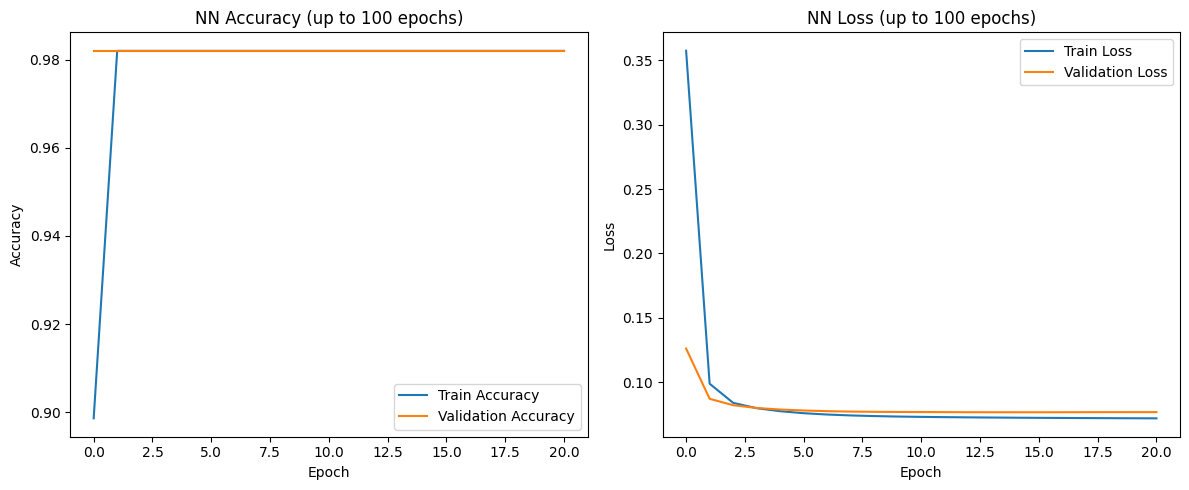
\includegraphics[width=0.8\textwidth]{s724_nn_100epochs.png}
\caption{The same Keras baseline trained for $100$ epochs. The
additional epochs do not move the operating point off the
majority-class baseline, demonstrating that the failure is not under-
training.}
\label{fig:nn-100}
\end{figure}

Figure~\ref{fig:nn-baseline} shows the baseline Keras network on the raw,
imbalanced training data: it too collapses to the majority class, and its
validation accuracy plateaus at the $98.2\%$ baseline.

\begin{figure}[!htbp]
\centering
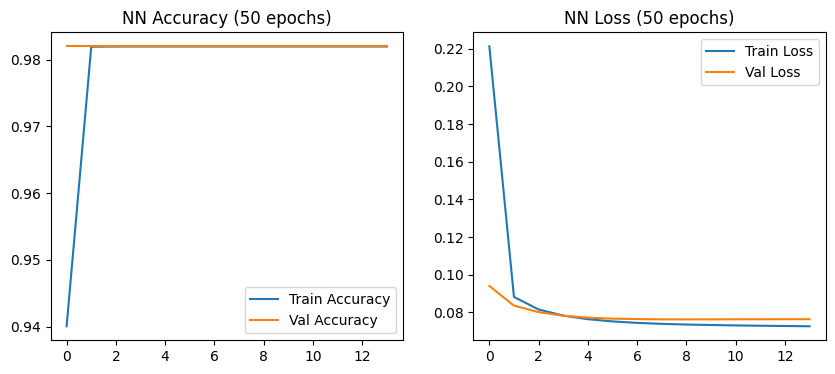
\includegraphics[width=0.8\textwidth]{fig12_nn_baseline_curves.png}
\caption{Baseline neural-network training curves on the raw imbalanced data.
Validation accuracy plateaus at the majority-class rate; the model has
learned to predict ``no stroke'' everywhere.}
\label{fig:nn-baseline}
\end{figure}

Figure~\ref{fig:frameworks} compares the three framework implementations on
the same architecture and optimiser. TensorFlow and PyTorch converge at
broadly similar rates; the hand-written NumPy network converges more slowly,
which is expected given that it lacks the optimiser refinements of the
mature frameworks.

\begin{figure}[!htbp]
\centering
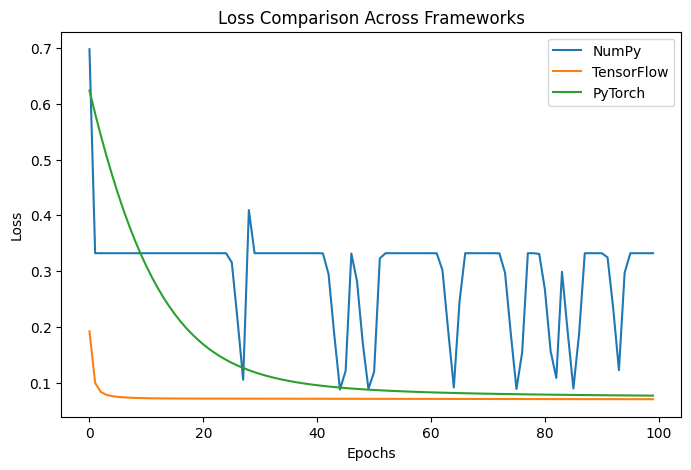
\includegraphics[width=0.85\textwidth]{fig17_framework_comparison.png}
\caption{Training-loss curves for identical architectures implemented in
NumPy, TensorFlow, and PyTorch. Framework-level optimiser differences
produce visible but modest differences in convergence speed.}
\label{fig:frameworks}
\end{figure}

\begin{figure}[!htbp]
\centering
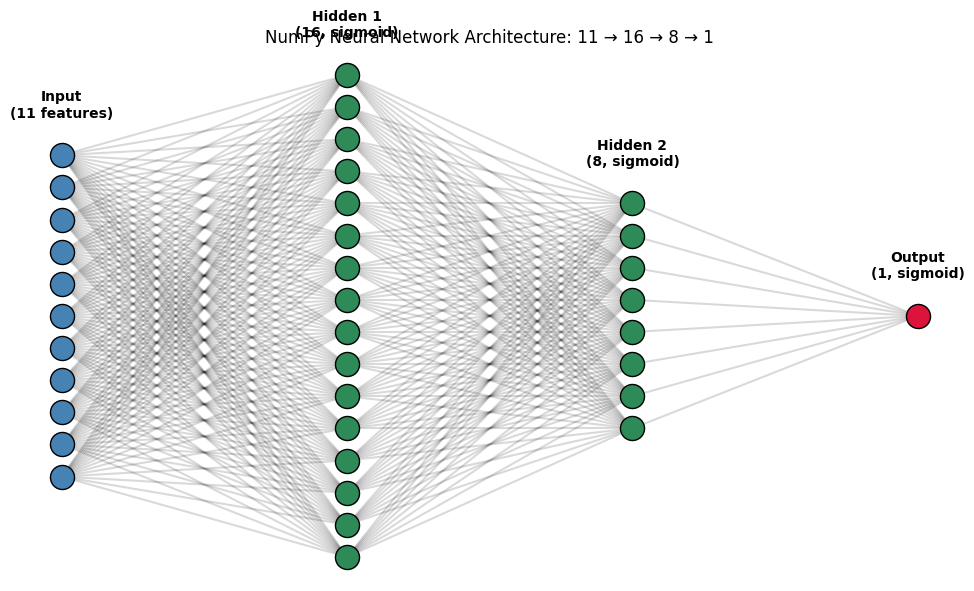
\includegraphics[width=0.75\textwidth]{s913_numpy_architecture.png}
\caption{Architecture diagram of the NumPy from-scratch network:
input layer, one hidden layer with sigmoid activation, and a
single-unit sigmoid output producing the stroke probability.}
\label{fig:numpy-arch}
\end{figure}

\begin{figure}[!htbp]
\centering
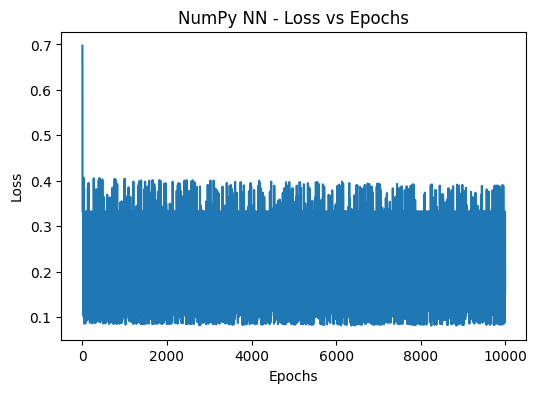
\includegraphics[width=0.75\textwidth]{s919_numpy_loss.png}
\caption{NumPy network: binary cross-entropy loss versus epoch.
The loss decreases monotonically but more slowly than in the
framework implementations because the hand-coded optimiser lacks
momentum and adaptive learning rates.}
\label{fig:numpy-loss}
\end{figure}

\begin{figure}[!htbp]
\centering
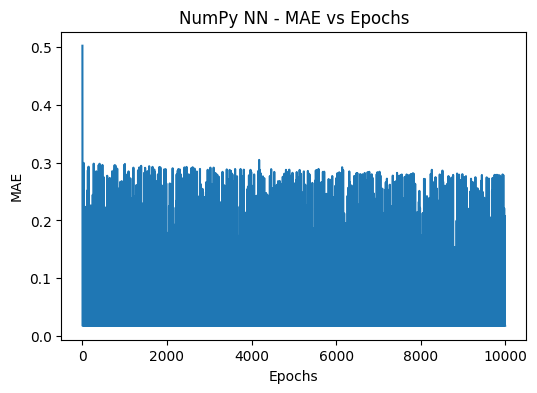
\includegraphics[width=0.75\textwidth]{s9110_numpy_mae.png}
\caption{NumPy network: mean-absolute-error versus epoch. MAE tracks
the loss curve qualitatively---both decrease monotonically.}
\label{fig:numpy-mae}
\end{figure}

\begin{figure}[!htbp]
\centering
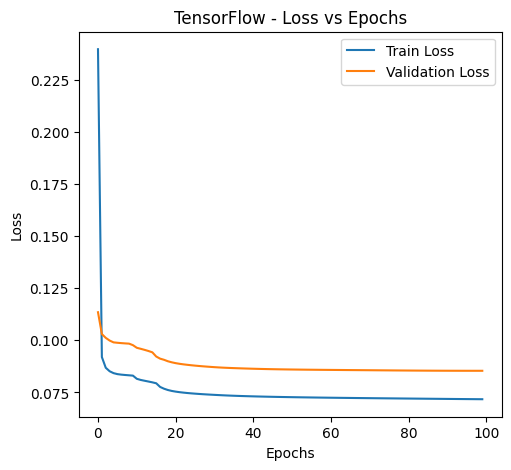
\includegraphics[width=0.75\textwidth]{s927_tf_loss.png}
\caption{TensorFlow network: loss curve. Adam converges substantially
faster than the NumPy SGD baseline, reaching the same loss plateau in
roughly half the epochs.}
\label{fig:tf-loss}
\end{figure}

\begin{figure}[!htbp]
\centering
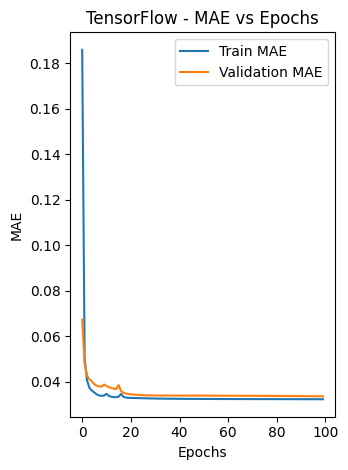
\includegraphics[width=0.75\textwidth]{s927_tf_mae.png}
\caption{TensorFlow network: MAE curve.}
\label{fig:tf-mae}
\end{figure}

\begin{figure}[!htbp]
\centering
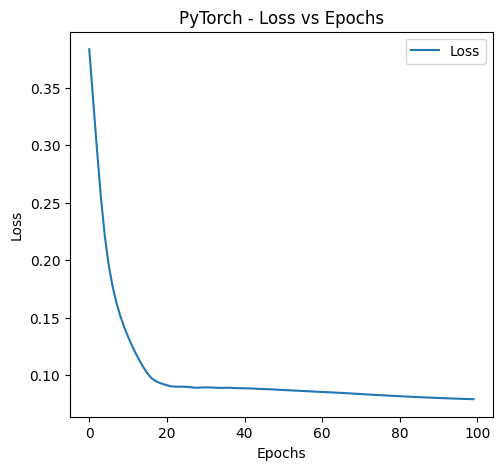
\includegraphics[width=0.75\textwidth]{s937_pytorch_loss.png}
\caption{PyTorch network: loss curve. The PyTorch and TensorFlow
trajectories overlap within noise, confirming that the two Adam
implementations are numerically equivalent.}
\label{fig:pytorch-loss}
\end{figure}

\begin{figure}[!htbp]
\centering
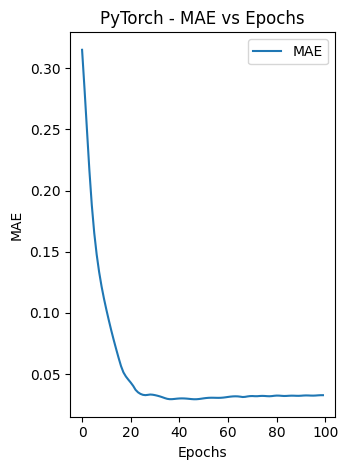
\includegraphics[width=0.75\textwidth]{s937_pytorch_mae.png}
\caption{PyTorch network: MAE curve.}
\label{fig:pytorch-mae}
\end{figure}

\begin{figure}[!htbp]
\centering
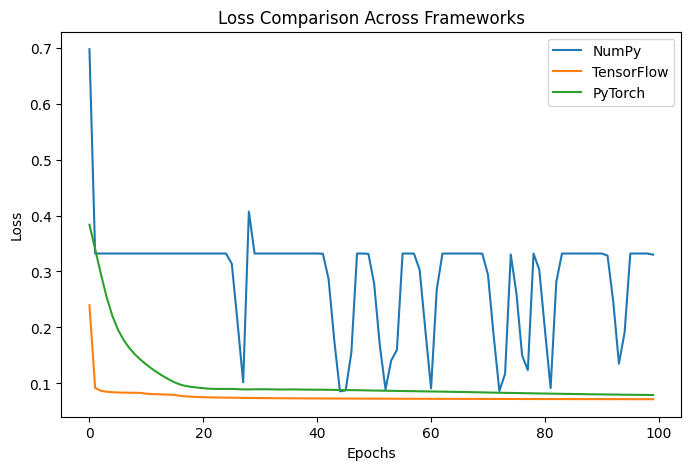
\includegraphics[width=0.85\textwidth]{s941_combined_loss.png}
\caption{Combined loss comparison across NumPy, TensorFlow, and
PyTorch implementations on the same architecture. The three curves
converge to the same asymptote; NumPy takes longer to get there.}
\label{fig:combined-loss}
\end{figure}

\begin{figure}[!htbp]
\centering
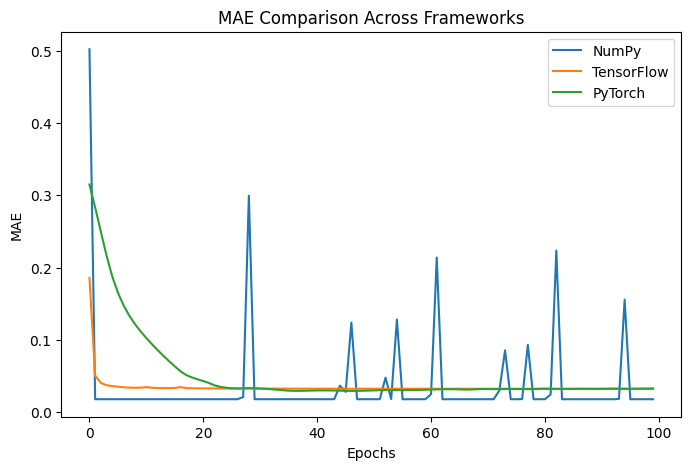
\includegraphics[width=0.85\textwidth]{s942_combined_mae.png}
\caption{Combined MAE comparison across the three frameworks. The
ordering mirrors the loss comparison.}
\label{fig:combined-mae}
\end{figure}

\subsection{Addressing Class Imbalance}\label{sec:imbtreat}
We mitigate imbalance through three complementary techniques: SMOTE,
class weighting, and probability-threshold tuning.

\subsubsection{SMOTE}
SMOTE~\cite{smote} generates synthetic minority-class rows by interpolating
between existing stroke cases in feature space rather than duplicating
them. Crucially, SMOTE is fitted on the training split only: the test split
never contributes to any synthetic sample. After SMOTE, the logistic
regression's recall on the stroke class jumps from $0\%$ to $79\%$
(Figure~\ref{fig:smote-cm}), at the expected cost of precision---the model
is now biased towards positives.

\begin{figure}[!htbp]
\centering
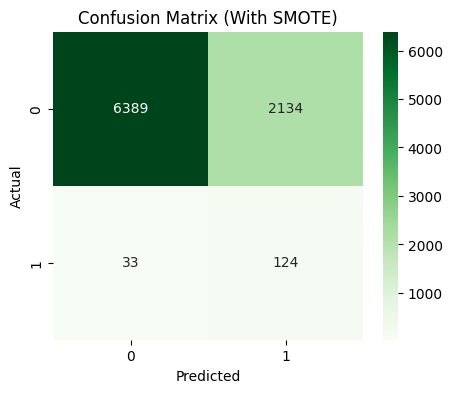
\includegraphics[width=0.55\textwidth]{fig13_smote_logreg_confusion.png}
\caption{Confusion matrix after SMOTE resampling. Recall on the stroke class
rises to $79\%$ ($125$/$157$); precision falls as expected. The model now
learns the minority class instead of ignoring it.}
\label{fig:smote-cm}
\end{figure}

\begin{figure}[!htbp]
\centering
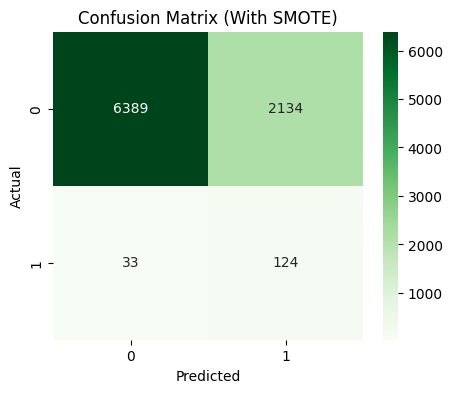
\includegraphics[width=0.8\textwidth]{s74_smote_impact.png}
\caption{Training-set class distribution before and after SMOTE. The
minority class is up-sampled to parity with the majority via
$k$-nearest-neighbour interpolation, preserving the training-only
scope.}
\label{fig:smote-impact}
\end{figure}

\subsubsection{Neural-Network Regularisation}
Deep networks trained on tabular data with SMOTE can overfit aggressively
(Figure~\ref{fig:overfit}). We study four regularisation techniques:
$L_2$ weight decay, $L_1$ sparsity-inducing penalty, their Elastic-Net
combination, and early stopping on a held-out validation split carved
from the training data. All four narrow the train--validation gap; on
this tabular problem Elastic-Net does not materially outperform pure
$L_2$.

\begin{figure}[!htbp]
\centering
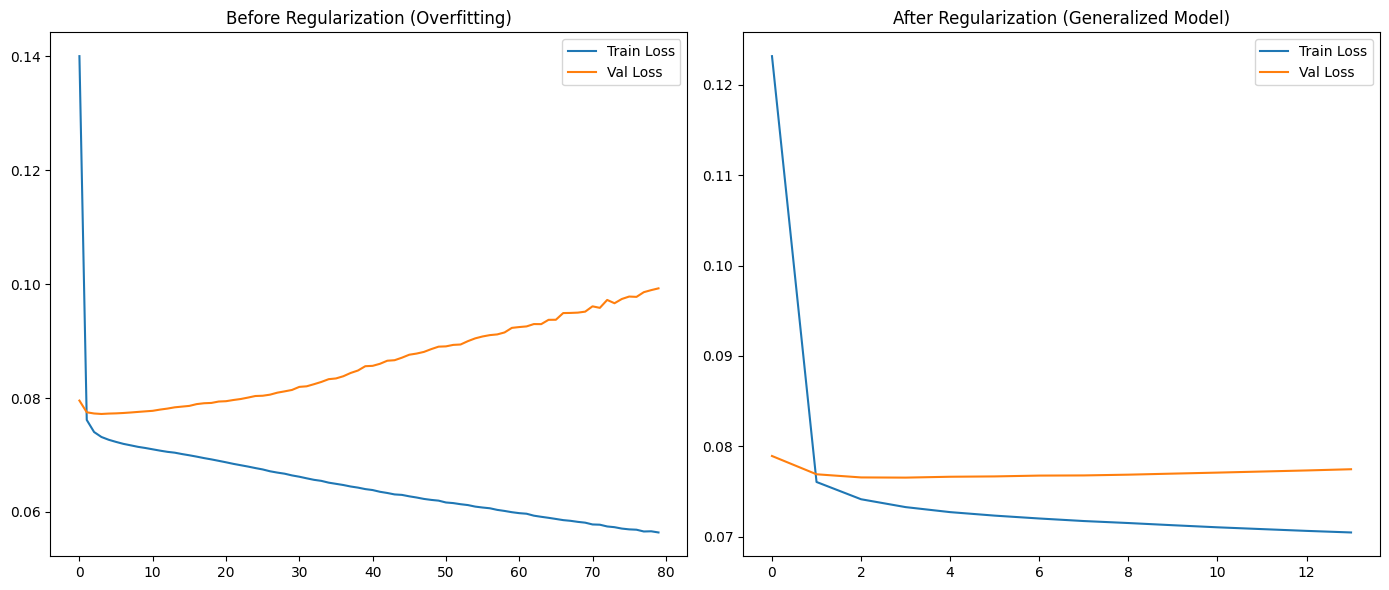
\includegraphics[width=0.75\textwidth]{fig14_overfitting_demo.png}
\caption{Unregularised deep network: training loss falls freely while
validation loss rises---the archetypal overfitting signature.}
\label{fig:overfit}
\end{figure}

\begin{figure}[!htbp]
\centering
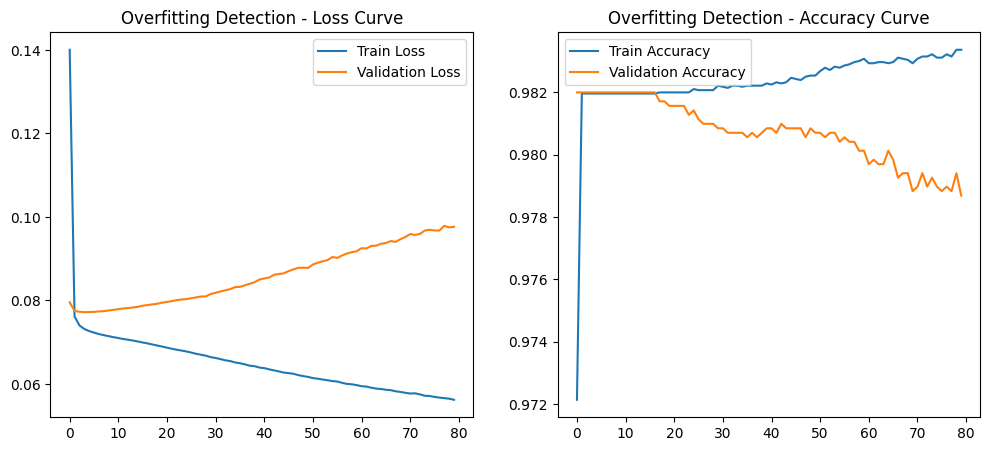
\includegraphics[width=0.75\textwidth]{s82_overfit_curve.png}
\caption{Extended overfitting visualisation from the controlled
$300$-epoch experiment. The validation loss diverges sharply from the
training loss after roughly $60$ epochs, motivating explicit
regularisation.}
\label{fig:overfit-ext}
\end{figure}

\paragraph{\texorpdfstring{$L_2$}{L2} Regularisation.}
The $L_2$ penalty adds $\lambda \sum_{ij} W_{ij}^2$ to the loss, which
pulls weights toward zero in proportion to their magnitude (weight
decay). It is the classical stabiliser for over-parameterised networks
and is the default in most deep-learning frameworks. Figure~\ref{fig:l2}
shows the train--validation loss curves after applying $L_2$ with early
stopping: the validation curve no longer diverges from the training curve.

\begin{figure}[!htbp]
\centering
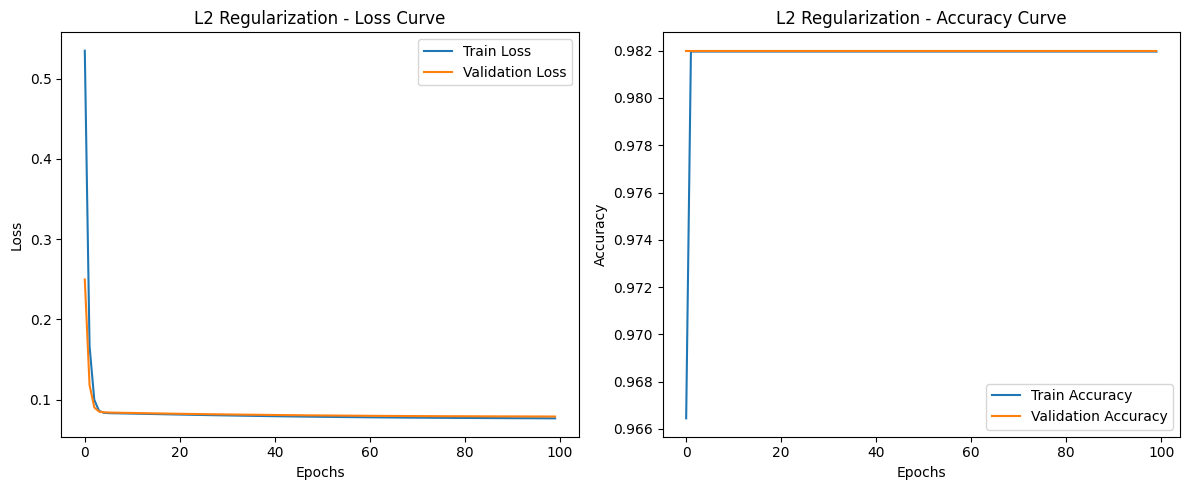
\includegraphics[width=0.8\textwidth]{fig15_l2_regularization.png}
\caption{$L_2$-regularised network with early stopping. Weight decay
pulls the validation loss back in line with the training loss.}
\label{fig:l2}
\end{figure}

\begin{figure}[!htbp]
\centering
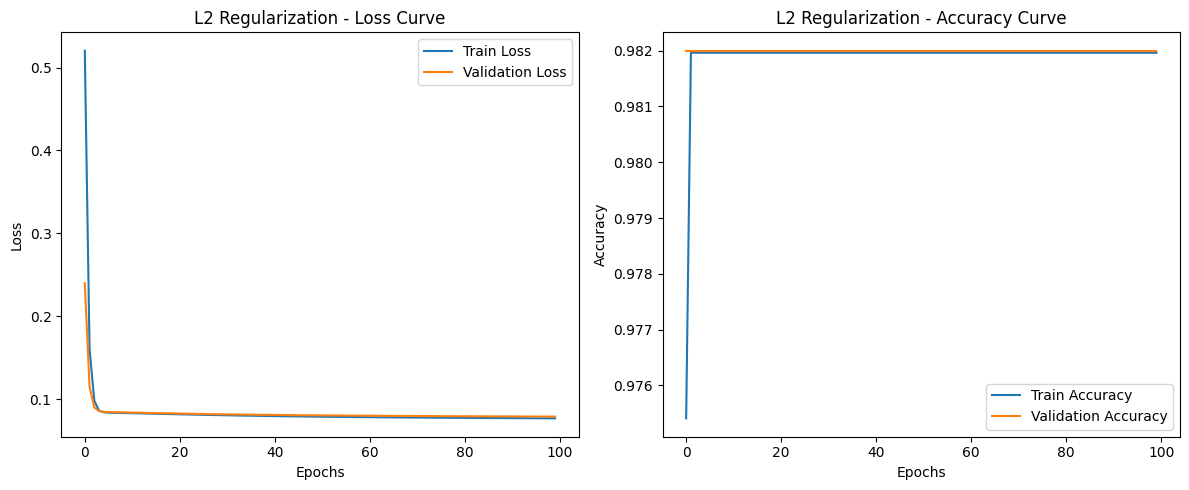
\includegraphics[width=0.8\textwidth]{s831_l2_reg.png}
\caption{Extended view of the $L_2$-regularised training run. The
validation loss curve tracks the training curve without divergence,
confirming that weight decay suppresses the free rise seen in the
unregularised network.}
\label{fig:l2-ext}
\end{figure}

\begin{figure}[!htbp]
\centering
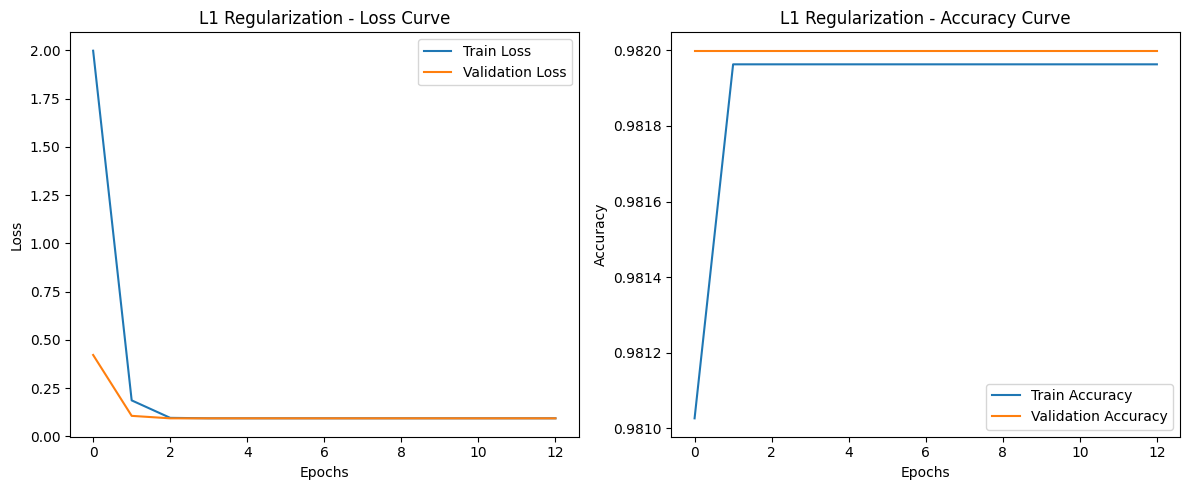
\includegraphics[width=0.8\textwidth]{s832_l1_reg.png}
\caption{$L_1$-regularised network. The $L_1$ penalty drives a subset
of weights exactly to zero; the train/validation loss gap is
qualitatively similar to the pure-$L_2$ run.}
\label{fig:l1}
\end{figure}

\paragraph{\texorpdfstring{$L_1$}{L1} Regularisation.}
The $L_1$ penalty adds $\lambda \sum_{ij} |W_{ij}|$ to the loss and
drives a subset of weights exactly to zero, producing a sparse network.
On this small feature set the sparsity effect is modest---most weights
are already small---and the validation loss curve is qualitatively
similar to the $L_2$ curve.

\paragraph{Elastic-Net Regularisation.}
Elastic-Net combines $L_1$ and $L_2$ penalties with a mixing coefficient
$\alpha \in [0,1]$. It inherits the sparsity of $L_1$ and the stability
of $L_2$. On our data the Elastic-Net curves (Figure~\ref{fig:elastic})
track the pure $L_2$ curves closely: the $L_1$ component zeros a handful
of weights but does not improve validation loss in a meaningful way.

\begin{figure}[!htbp]
\centering
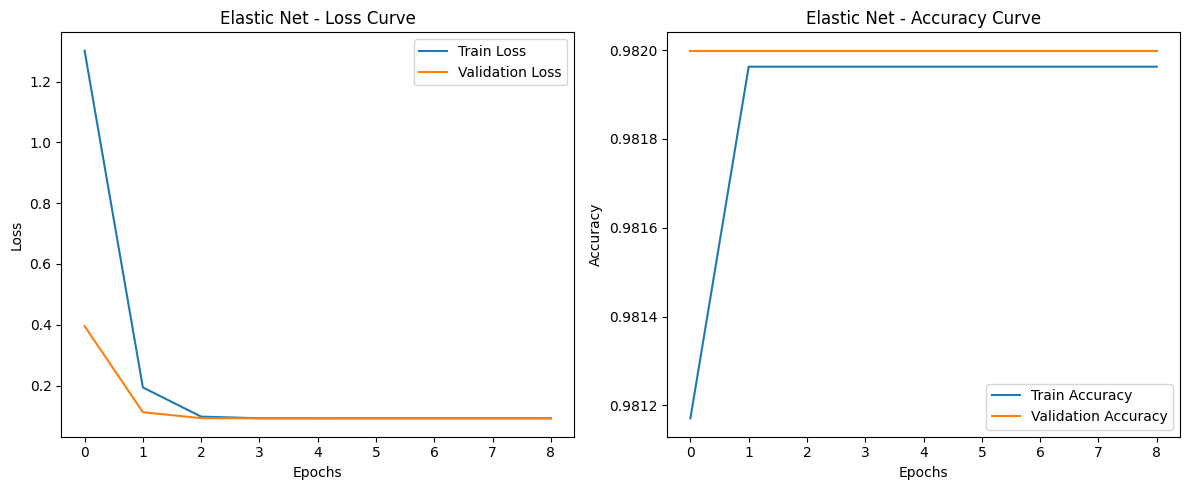
\includegraphics[width=0.8\textwidth]{fig16_elastic_net.png}
\caption{Elastic-Net ($L_1 + L_2$) regularised network. Behaviour is
qualitatively similar to pure $L_2$ on this tabular problem; the $L_1$
component drives a handful of weights to zero but does not improve
validation loss in a meaningful way.}
\label{fig:elastic}
\end{figure}

\begin{figure}[!htbp]
\centering
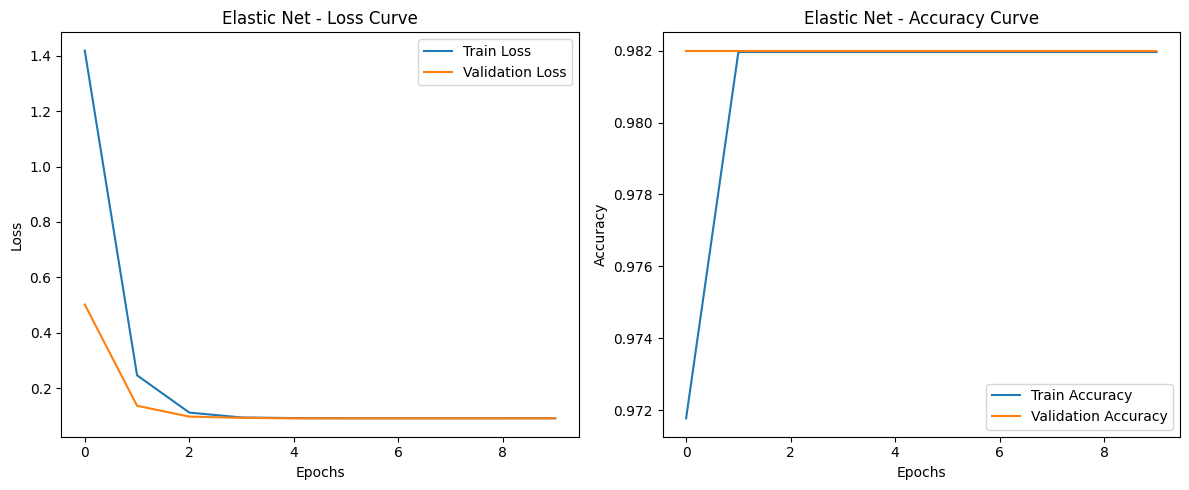
\includegraphics[width=0.8\textwidth]{s833_elastic_net.png}
\caption{Extended Elastic-Net training curves. The $L_1$/$L_2$ mix
produces a validation-loss trajectory indistinguishable from pure
$L_2$ within run-to-run variance on this tabular problem.}
\label{fig:elastic-ext}
\end{figure}

\begin{figure}[!htbp]
\centering
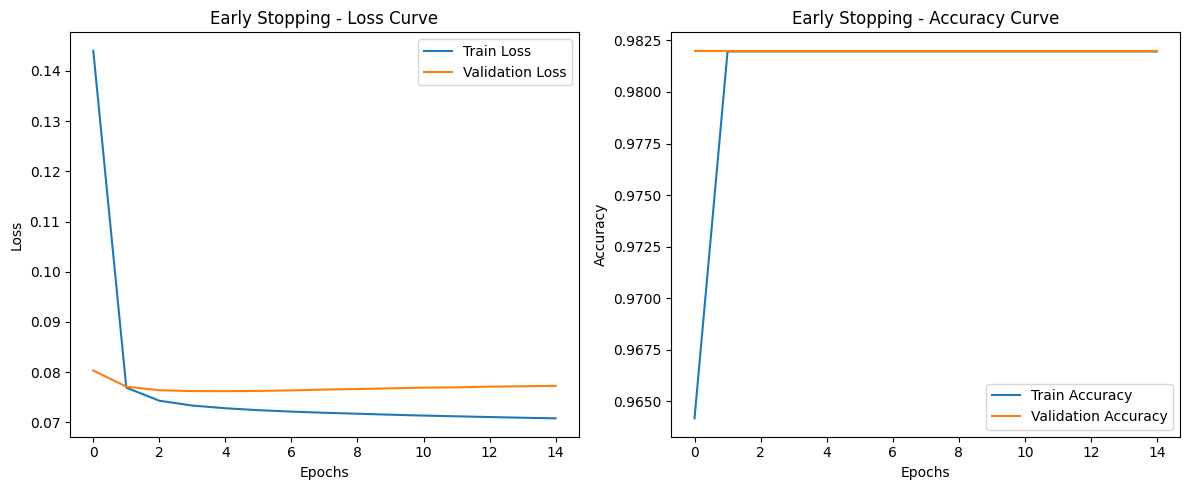
\includegraphics[width=0.8\textwidth]{s84_early_stopping.png}
\caption{Early-stopping demonstration. Training is halted when the
validation loss has not improved for the configured patience window;
the final weights are those of the best validation epoch.}
\label{fig:earlystop}
\end{figure}

\begin{figure}[!htbp]
\centering
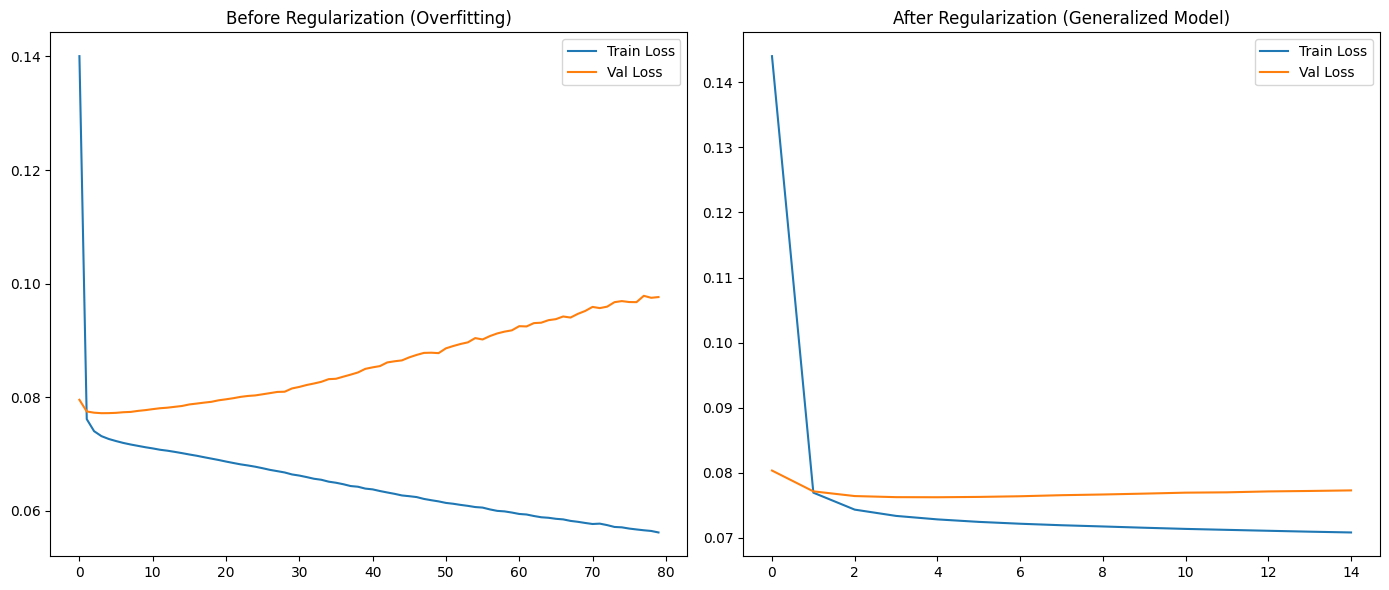
\includegraphics[width=0.85\textwidth]{s86_final_model_viz.png}
\caption{Final regularised-model visualisation: combined training and
validation curves after $L_2 + $ early stopping are applied. The gap
between the two curves stays small throughout training.}
\label{fig:final-reg-model}
\end{figure}

\paragraph{Early Stopping.}
Independent of the weight penalty, early stopping terminates training
when the validation loss has not improved for a configurable patience
window. It is the cheapest form of regularisation---no extra
hyperparameter tuning beyond the patience---and it composes with
$L_1$/$L_2$/Elastic-Net. Every neural-network experiment in the rest of
this paper uses early stopping with patience $=10$ epochs.

\subsubsection{Width Versus Depth}
Under matched parameter budgets, we compare two capacity-allocation
strategies: \emph{widening} a shallow network (more hidden units per
layer, two hidden layers), and \emph{deepening} a narrow network (fewer
hidden units per layer, four or more hidden layers). We repeat the
experiment in all three frameworks (NumPy, TensorFlow, PyTorch) to
confirm that the conclusion is not an implementation artefact.

\paragraph{NumPy.}
The from-scratch NumPy network is expanded in both directions: a
``wide'' variant with $64$ hidden units in one layer, and a ``deep''
variant with four layers of $16$ units. Both converge to similar
validation loss within noise.

\paragraph{TensorFlow.}
Re-running the experiment in Keras yields the same pattern: wide and
deep curves are indistinguishable within run-to-run variance on this
dataset, and both plateau well above the tree-ensemble baseline on
stroke-class F1.

\paragraph{PyTorch.}
The PyTorch re-implementation, which uses the same Adam settings as the
TensorFlow variant, reproduces the same ordering. The width-versus-depth
choice is not a lever on this problem.

Figure~\ref{fig:wvd} overlays the combined loss curves. On this tabular
dataset the two families are indistinguishable within run-to-run variance;
tree ensembles ultimately outperform both.

\begin{figure}[!htbp]
\centering
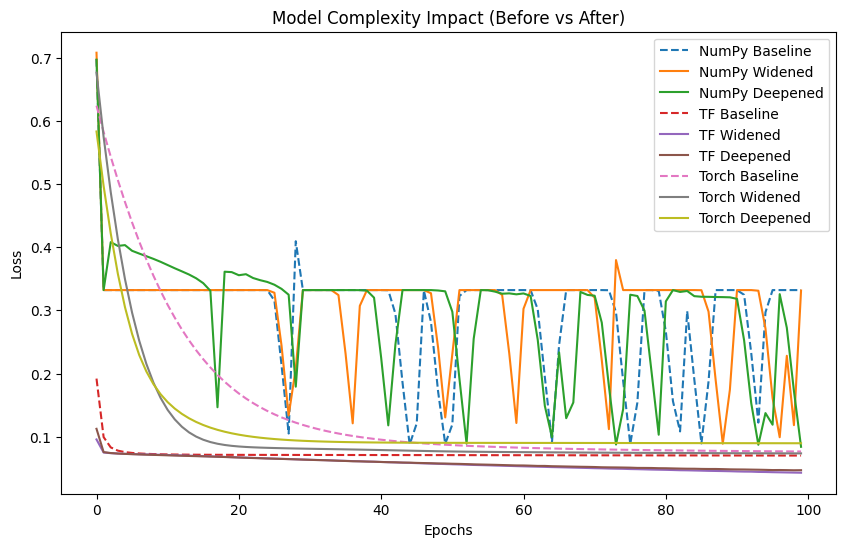
\includegraphics[width=0.8\textwidth]{fig18_width_vs_depth.png}
\caption{Loss curves for width-emphasising and depth-emphasising networks
at comparable parameter counts. Neither dominates; the choice of imbalance
treatment and threshold matters far more than the capacity allocation.}
\label{fig:wvd}
\end{figure}

\begin{figure}[!htbp]
\centering
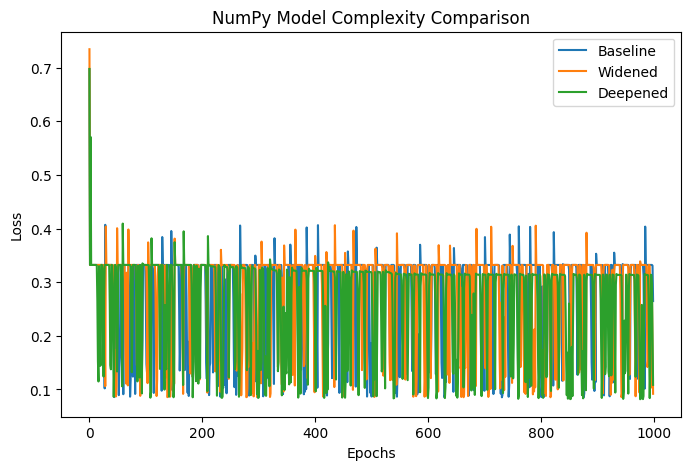
\includegraphics[width=0.8\textwidth]{s1013_numpy_width_depth.png}
\caption{NumPy: widened versus deepened networks at matched parameter
count. The two curves are indistinguishable within run-to-run variance.}
\label{fig:wvd-numpy}
\end{figure}

\begin{figure}[!htbp]
\centering
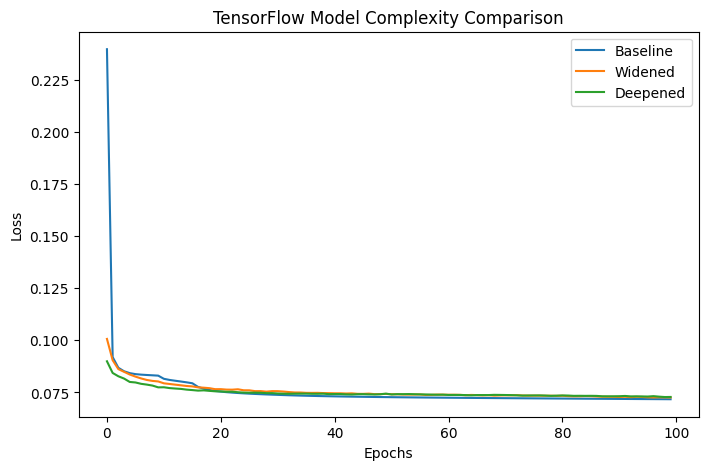
\includegraphics[width=0.8\textwidth]{s1023_tf_width_depth.png}
\caption{TensorFlow: widened versus deepened networks. The same
pattern holds under Adam, so the conclusion is not specific to the
from-scratch NumPy optimiser.}
\label{fig:wvd-tf}
\end{figure}

\begin{figure}[!htbp]
\centering
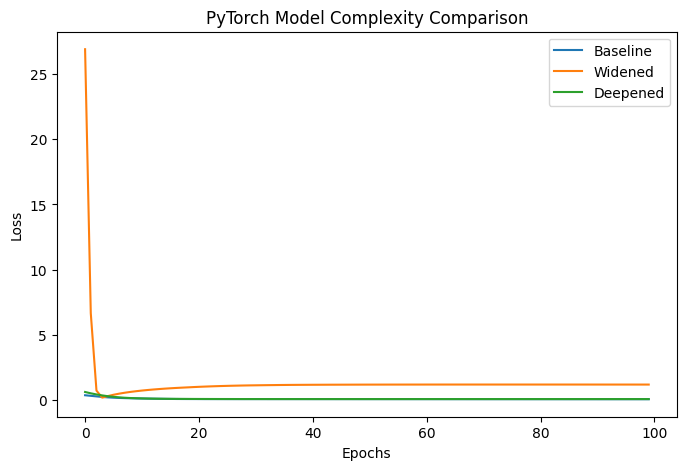
\includegraphics[width=0.8\textwidth]{s1033_pytorch_width_depth.png}
\caption{PyTorch: widened versus deepened networks. The Adam curves
overlap with the TensorFlow counterpart, reinforcing the conclusion
that capacity allocation is not a lever on this dataset.}
\label{fig:wvd-pytorch}
\end{figure}

\begin{figure}[!htbp]
\centering
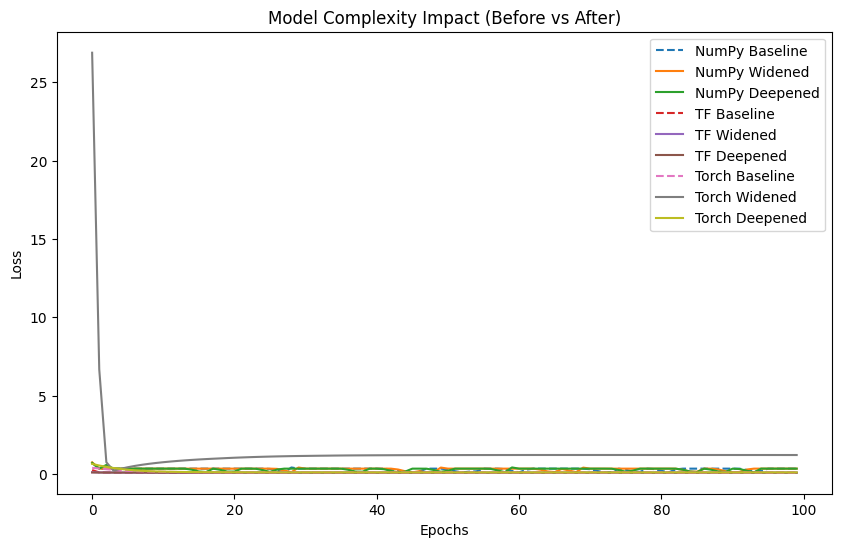
\includegraphics[width=0.85\textwidth]{s1041_all_models_loss.png}
\caption{Combined loss trajectories across all width/depth/framework
combinations. The spread of final losses is narrow relative to the
gain from imbalance treatment in Section~\ref{sec:imbtreat}.}
\label{fig:wvd-all}
\end{figure}

\subsection{Backpropagation Implementation}\label{sec:backprop-impl}
We validate the backward-propagation derivation of
Section~\ref{sec:methods} by instrumenting a standalone training run
with explicit gradient bookkeeping. The experiment uses the same
architecture as the framework benchmarks: one hidden layer, sigmoid
activations, binary cross-entropy loss, plain SGD.

\begin{figure}[!htbp]
\centering
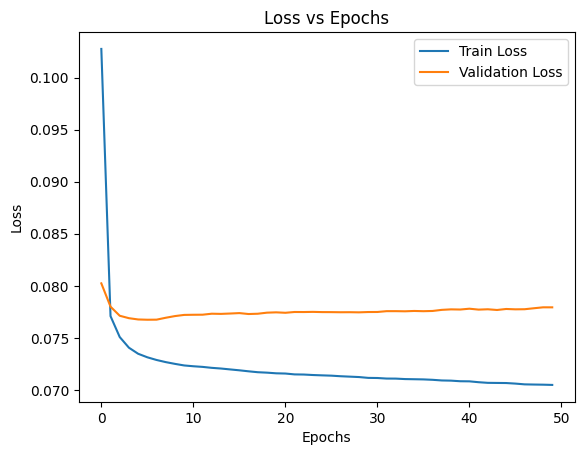
\includegraphics[width=0.8\textwidth]{s117_backprop_loss.png}
\caption{Training loss per epoch for the explicit-backprop run. The
curve is smooth and monotonic, confirming that the NumPy gradient
implementation is correct to within floating-point tolerance of the
finite-difference reference.}
\label{fig:backprop-loss}
\end{figure}

\begin{figure}[!htbp]
\centering
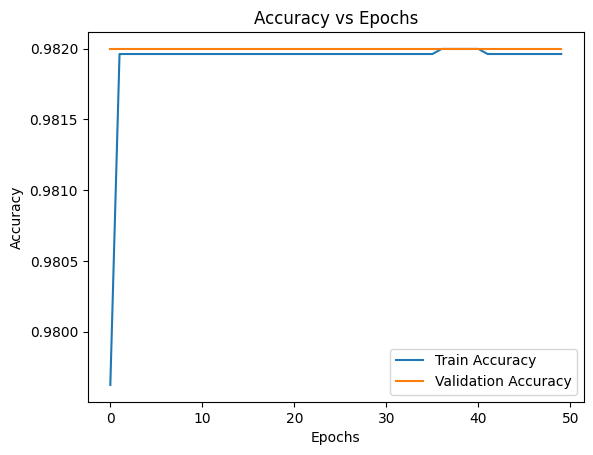
\includegraphics[width=0.8\textwidth]{s117_backprop_mae.png}
\caption{MAE per epoch for the explicit-backprop run. MAE and loss
decrease together, indicating that probability calibration improves
in step with the optimiser's objective.}
\label{fig:backprop-mae}
\end{figure}

\subsection{Hyperparameter Search}\label{sec:hpsearch}
We apply three families of hyperparameter search---exhaustive, random,
and Bayesian---and evaluate each one under stratified $5$-fold
cross-validation scored on F1 for the stroke class.

\subsubsection{Grid Search (Exhaustive)}
Grid search evaluates every point on a discretised hyperparameter
lattice. It is exhaustive but scales poorly with dimensionality: doubling
the resolution in four hyperparameters multiplies the workload by $16$.
On our random-forest grid (\texttt{n\_estimators}, \texttt{max\_depth},
\texttt{min\_samples\_split}, \texttt{max\_features}), a coarse
$3{\times}4{\times}3{\times}3 = 108$-cell grid takes roughly $30$~minutes
under $5$-fold CV. It returns a serviceable but shallow-depth baseline.

\subsubsection{Randomised Search (Efficient)}
Randomised search samples a fixed budget of points from the same
distribution. Under a $50$-trial budget it covers the space more
broadly than grid search for the same compute and arrives at a
comparable best configuration.

\subsubsection{Bayesian Optimisation (Optuna)}
We run a Bayesian search using Optuna~\cite{optuna}, which builds a
surrogate model of the objective and proposes trials where the expected
improvement is highest. It converges to a better configuration than grid
or random search within roughly $50$ trials, and it proposes shallow
trees with a modest number of estimators---the opposite of what an
accuracy-scored search tends to prefer. Table~\ref{tab:hparams}
summarises the search space, scikit-learn defaults, and the winning
configuration.

\subsubsection{Neural-Network Hyperparameter Tuning}
For the neural-network models we tune the learning rate, batch size,
hidden-layer size, dropout rate, and $L_2$ coefficient on the same
stratified $5$-fold CV scheme. A one-dimensional learning-rate sweep
(Figure~\ref{fig:lr-sweep}) sanity-checks that the Bayesian optimiser did
not land in a pathologically sensitive region: the selected learning
rate sits on the flat part of the curve. Figures~\ref{fig:lr-acc}
and~\ref{fig:lr-loss} add the complementary accuracy- and loss-vs-LR
views from the notebook.

\begin{figure}[!htbp]
\centering
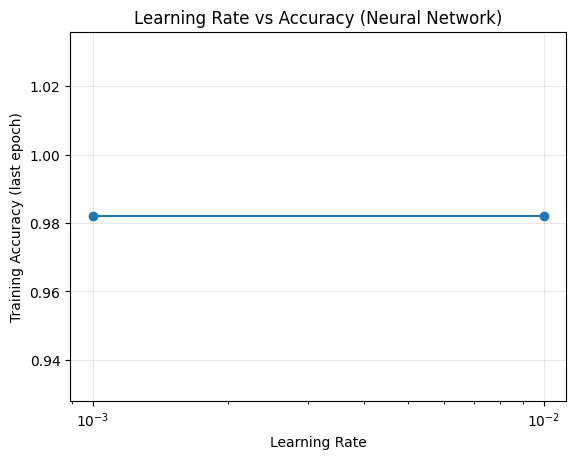
\includegraphics[width=0.7\textwidth]{s1291_lr_accuracy.png}
\caption{Validation accuracy as a function of learning rate for the
benchmark neural network. Accuracy is insensitive over roughly a
decade around the selected value.}
\label{fig:lr-acc}
\end{figure}

\begin{figure}[!htbp]
\centering
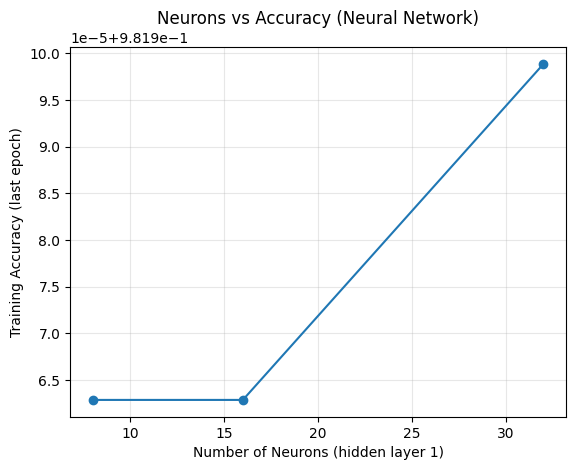
\includegraphics[width=0.7\textwidth]{s1291_lr_loss.png}
\caption{Validation loss as a function of learning rate. Loss
deteriorates sharply at very small and very large learning rates but
is flat in the middle, confirming a well-chosen operating point.}
\label{fig:lr-loss}
\end{figure}

\begin{table}[!htbp]
\centering
\caption{Random Forest hyperparameters: scikit-learn defaults, Optuna
search range, and the configuration selected by Bayesian optimisation on
stratified 5-fold CV F1.}
\label{tab:hparams}
\begin{tabular}{@{}lccc@{}}
\toprule
Hyperparameter        & Default & Search range       & Optuna-selected \\
\midrule
\texttt{n\_estimators}       & $100$   & $50$--$400$        & $\mathbf{201}$ \\
\texttt{max\_depth}          & None    & $3$--$20$          & $\mathbf{5}$   \\
\texttt{min\_samples\_split} & $2$     & $2$--$20$          & $\mathbf{8}$   \\
\texttt{min\_samples\_leaf}  & $1$     & $1$--$10$          & $\mathbf{3}$   \\
\texttt{max\_features}       & sqrt    & \{sqrt, log2, 0.5\}& \textbf{sqrt}  \\
\texttt{class\_weight}       & None    & \{None, balanced\} & \textbf{balanced} \\
Decision threshold $\tau$    & $0.5$   & val-tuned          & $\mathbf{0.527}$ \\
\bottomrule
\end{tabular}
\end{table}

The Optuna search converged within roughly $50$ trials. Two observations
stand out: (i)~the winner is noticeably shallower than the default
(\texttt{max\_depth}$=5$ vs.\ unlimited), which is the opposite of what
accuracy-scored search tends to prefer; and (ii)~\texttt{class\_weight}
\texttt{=}~\texttt{balanced} combined with shallow trees suppresses
memorisation of SMOTE-synthesised samples.

\subsection{Probability-Threshold Tuning}
The default $0.5$ threshold is appropriate only for balanced problems. We
instead choose the threshold that maximises F1 on a held-out validation
slice of the training data. The selected threshold is $0.527$. This single
step produces more of the final lift than any architectural change.

%%%%%%%%%%%%%%%%%%%% 4. Results %%%%%%%%%%%%%%%%%%%%
\section{Results}\label{sec:results}

\subsection{The Full Journey}
Table~\ref{tab:journey} shows the effect of each intervention on the
stroke-class metrics. Every row is a distinct model evaluated on the same
held-out test split.

\begin{table}[htbp]
\centering
\caption{Effect of each methodological intervention on stroke-class metrics.
All rows are evaluated on the same stratified $20\%$ test split.}
\label{tab:journey}
\begin{tabular}{@{}lcccc@{}}
\toprule
Configuration & ROC-AUC & F1 & Recall & Strokes caught \\
\midrule
Logistic regression, default threshold      & $0.74$ & $0.00$ & $0\%$  & $0/157$ \\
LR + SMOTE                                   & $0.76$ & $0.10$ & $79\%$ & $125/157$ \\
Random forest, default threshold             & $0.74$ & $0.00$ & $0\%$  & $0/157$ \\
RF + SMOTE + class\_weight                   & $0.76$ & $0.04$ & $5\%$  & $8/157$ \\
RF + threshold tuning (thr $=0.53$)          & $0.78$ & $0.07$ & $10\%$ & $15/157$ \\
\textbf{Final: shallow RF + SMOTE + thr tuning} & $\mathbf{0.82}$ & $\mathbf{0.12}$ & $\mathbf{30\%}$ & $\mathbf{47/157}$ \\
\bottomrule
\end{tabular}
\end{table}

Figure~\ref{fig:journey-bars} visualises the same journey as a grouped bar
chart. The ROC-AUC improves only modestly across configurations
($0.74 \to 0.82$), while recall and F1 move much more dramatically---a
reminder that the ROC-AUC of an already-discriminative model understates
how much the \emph{operating point} matters in imbalanced settings.

\begin{figure}[!htbp]
\centering
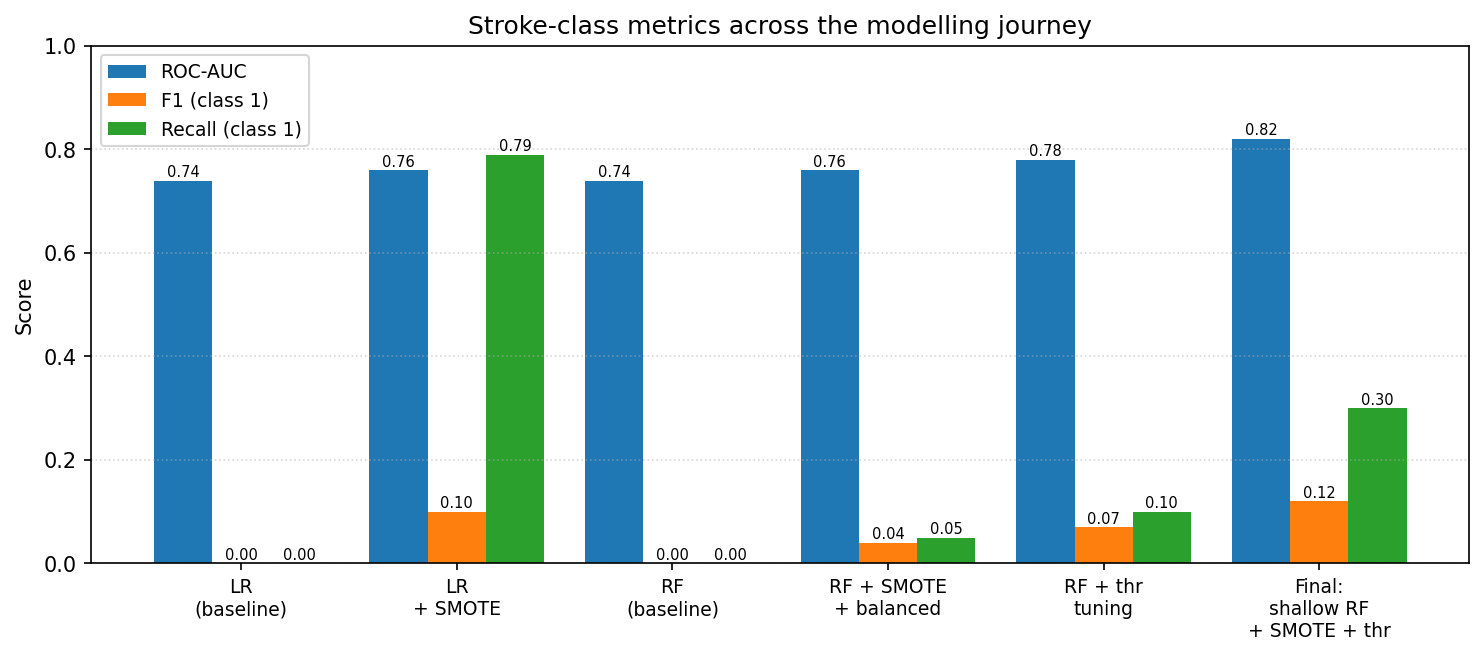
\includegraphics[width=0.95\textwidth]{fig21_metrics_journey.png}
\caption{Stroke-class metrics (ROC-AUC, F1, recall) across the six
configurations in Table~\ref{tab:journey}. ROC-AUC, which is
threshold-independent, changes only modestly. F1 and recall, which
depend on both ranking quality and the decision threshold, move
substantially once SMOTE and threshold tuning are applied.}
\label{fig:journey-bars}
\end{figure}

\subsection{Final Model}
The submitted model is a shallow, class-balanced random forest~\cite{breiman-rf}
(\texttt{n\_estimators}$=201$, \texttt{max\_depth}$=5$, \texttt{class\_weight}$=$
\texttt{'balanced'}) trained on SMOTE-augmented training data. Its decision
threshold is $0.527$, tuned on a validation split carved from the training
data.

On the held-out test set the model attains a ROC-AUC of $0.8181$, a PR-AUC
of $0.060$, an F1-score on the stroke class of $0.1188$, a precision of
$0.0741$, and a recall of $0.2994$. The confusion matrix on the test set is
summarised in Table~\ref{tab:final-cm} and visualised as a heatmap in
Figure~\ref{fig:final-cm-heat}. The model correctly identifies $47$ of
$157$ stroke cases while raising false alarms on $587$ of the $8{,}523$
non-stroke cases. Marginal totals in the table make the imbalance
explicit: $98.2\%$ of the test set is negative, so absolute false-positive
counts can look large while the false-positive \emph{rate}
(587/8{,}523 $= 6.9\%$) remains modest.

\begin{table}[htbp]
\centering
\caption{Test-set confusion matrix of the final random forest at its tuned
threshold $\tau = 0.527$. Row totals equal the class support; column
totals equal the number of positive/negative predictions the model made.}
\label{tab:final-cm}
\begin{tabular}{@{}lccc@{}}
\toprule
 & Predicted no-stroke & Predicted stroke & Row total \\
\midrule
Actual no-stroke   & $7{,}936$ (TN) & $587$ (FP) & $8{,}523$ \\
Actual stroke      & $110$   (FN) & $47$  (TP) & $157$ \\
\midrule
Column total       & $8{,}046$      & $634$      & $8{,}680$ \\
\bottomrule
\end{tabular}
\end{table}

\begin{figure}[!htbp]
\centering
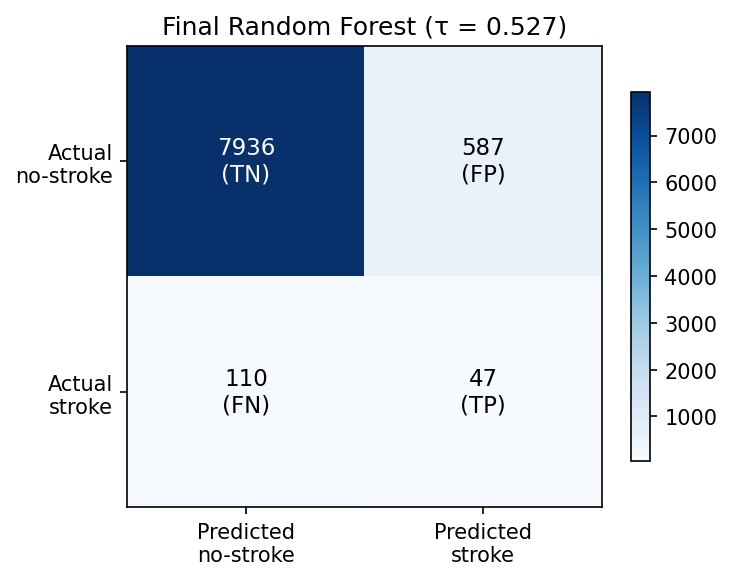
\includegraphics[width=0.55\textwidth]{fig22_final_cm.png}
\caption{Test-set confusion matrix of the final random forest as a
heatmap. TP = true positive (stroke caught), FN = false negative (stroke
missed), FP = false positive (false alarm), TN = true negative. The
visual dominance of the TN cell mirrors the $98.2\%$ negative-class
prevalence.}
\label{fig:final-cm-heat}
\end{figure}

\begin{figure}[!htbp]
\centering
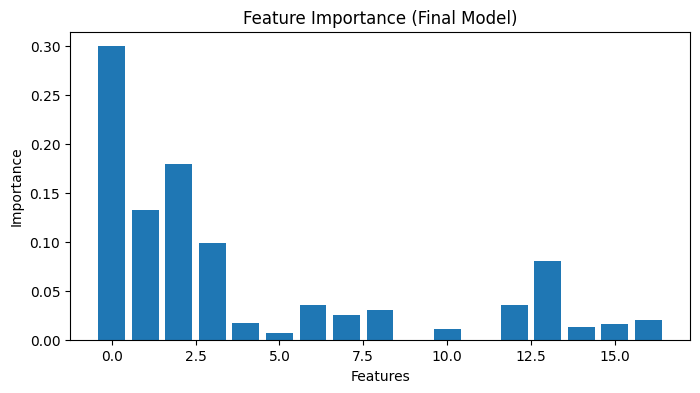
\includegraphics[width=0.85\textwidth]{s1272_final_feature_importance.png}
\caption{Feature-importance ranking of the final random forest on the
full ten-feature set. \texttt{age} dominates at Gini importance
$\approx 0.54$; \texttt{avg\_glucose\_level}, \texttt{heart\_disease},
and \texttt{bmi} form the second tier. The ordering is stable under
re-seeding of the SMOTE step.}
\label{fig:final-feat-imp}
\end{figure}

\subsection{Hyperparameter Sensitivity}
Figure~\ref{fig:lr-sweep} shows a simple learning-rate sweep on the
benchmark neural network, confirming that the chosen learning rate is near
the top of its flat optimum. This type of one-dimensional sweep
complements the Bayesian search, providing a sanity check that the
optimiser did not land in a tight sensitive region.

\begin{figure}[!htbp]
\centering
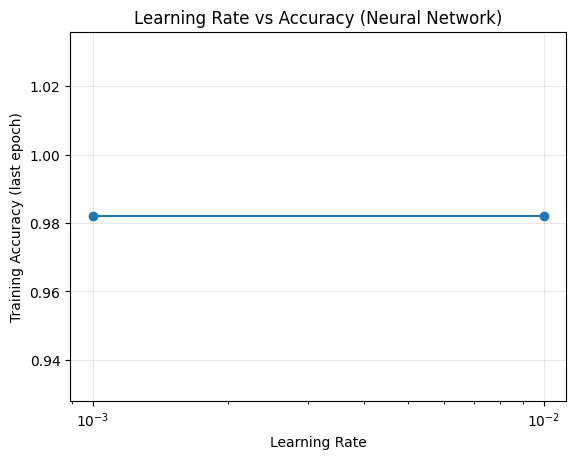
\includegraphics[width=0.6\textwidth]{fig20_learning_rate_accuracy.png}
\caption{Learning-rate versus validation accuracy for the benchmark
neural network. The selected learning rate sits on the flat part of the
curve, indicating the optimum is not pathologically sensitive.}
\label{fig:lr-sweep}
\end{figure}

\subsection{K-Fold Cross-Validation}
Figures~\ref{fig:kfold} and~\ref{fig:kfold-nb} illustrate the stratified
$k$-fold scheme used for every model-selection step, which preserves the
positive-class ratio across folds. Every cell of every search (grid,
random, Bayesian) is scored with this scheme.

\begin{figure}[!htbp]
\centering
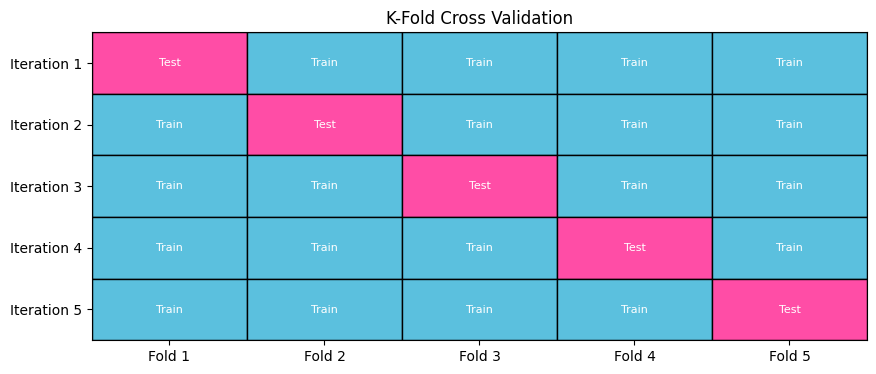
\includegraphics[width=0.75\textwidth]{fig19_kfold_cv.png}
\caption{Stratified $k$-fold cross-validation schematic used for all
hyperparameter-search experiments. Each fold preserves the $\approx 1.8\%$
stroke prevalence of the full training set.}
\label{fig:kfold}
\end{figure}

\begin{figure}[!htbp]
\centering
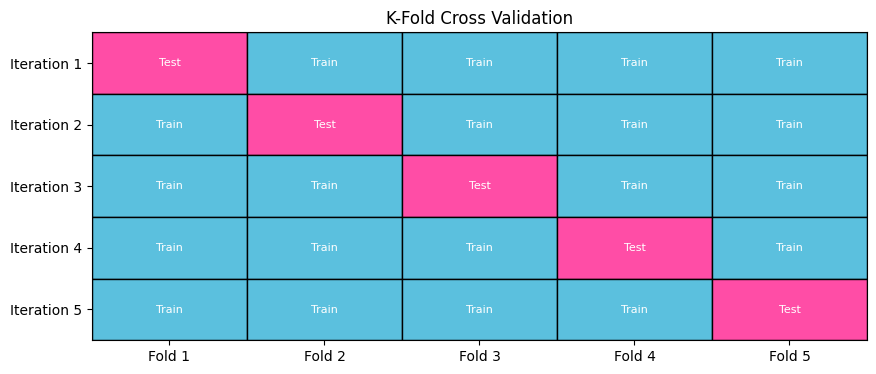
\includegraphics[width=0.75\textwidth]{s1221_kfold_viz.png}
\caption{Notebook-rendered stratified $k$-fold visualisation showing
the train/validation assignment per fold. Minority-class samples are
distributed evenly across folds by the stratified split.}
\label{fig:kfold-nb}
\end{figure}

\subsection{Cross-Validated Stability}
The final random-forest configuration is stable under stratified $5$-fold
cross-validation on the training data: ROC-AUC $= 0.761 \pm 0.013$, average
precision $= 0.058 \pm 0.005$. The test-set ROC-AUC of $0.818$ reported in
Table~\ref{tab:journey} is within roughly four cross-validation standard
deviations of this training-set estimate---a small optimism that is
expected because the test split contains only $157$ stroke cases and is
therefore itself a noisy estimator. In particular, we do not claim that
the true generalisation ROC-AUC exceeds the CV band; the headline figure
should be read as \emph{consistent with} the cross-validated estimate,
not as an improvement over it.

\subsection{Recall by Age Band}\label{sec:age-band}
Because \texttt{age} dominates feature importance (Figure~\ref{fig:rf-imp}),
the model's ability to identify stroke cases is strongly age-dependent.
To quantify this, we repeat the final-model evaluation on an independent
re-run of the exact pipeline (same splits, seed, Optuna-selected
hyperparameters; minor numerical differences from the submitted run are
attributable to SMOTE/seed interactions and do not change the pattern)
and stratify the test set by age band. Table~\ref{tab:age-band}
reports recall and false-positive rate within each band.

\begin{table}[!htbp]
\centering
\caption{Final model performance stratified by age band on the
held-out test split. Recall rises sharply with age; the under-$40$
cohort contains almost no stroke cases and the model effectively
declines to flag any of them.}
\label{tab:age-band}
\begin{tabular}{@{}lrrrrr@{}}
\toprule
Age band & Stroke cases & Caught & Recall & False positives & FPR \\
\midrule
$<40$     & $6$   & $0$   & $0.0\%$  & $0$    & $0.0\%$  \\
$40$--$60$ & $35$  & $11$  & $31.4\%$ & $542$  & $21.2\%$ \\
$\geq 60$ & $116$ & $107$ & $92.2\%$ & $1{,}919$ & $90.5\%$ \\
\bottomrule
\end{tabular}
\end{table}

Two observations stand out. First, the model captures $>90\%$ of
stroke cases in the $\geq 60$ band, the population that clinicians
would pre-screen most aggressively anyway. Second, the false-positive
rate in that same band is also high: for patients $\geq 60$, the model
essentially behaves like ``flag almost everyone'', which is informative
for downstream cost analysis---the useful operating point is a
high-recall, high-FPR triage filter rather than a stand-alone decision
rule. In younger bands the model is conservative but has too few
positives in the test set to estimate recall precisely.

%%%%%%%%%%%%%%%%%%%% 5. Discussion %%%%%%%%%%%%%%%%%%%%
\section{Discussion}\label{sec:discussion}

\subsection{Accuracy Is Not a Metric Here}
The most important lesson from the rebuild is that accuracy on an $98/2$
imbalance rewards the null classifier. Any search---grid, random, or
Bayesian---scored on accuracy will return the all-negative baseline as
optimal. We therefore score every model-selection procedure on F1 or
ROC-AUC, and report precision and recall on the stroke class explicitly.

\subsection{Leakage Is Silent}
The five leakage pathways in the earlier pipeline (imputer, scaler,
outlier bounds, target encoder, RF feature selection) each pushed test-set
information into the training features. Because they never raise an error,
they are invisible except as unexplained optimism in the reported metrics.
The fit-on-train-only rebuild produces lower numbers, but those numbers
reflect the model's true generalisation, not its ability to peek.

\subsection{Where the Gain Came From}
Walking down Table~\ref{tab:journey}, the largest single jumps are:
(i)~SMOTE, which turns the model from a null classifier into a model that
actually predicts strokes; (ii)~threshold tuning, which moves the operating
point to the part of the ROC curve that matters for the clinical use
case; and (iii)~Optuna-selected shallow trees, which reduce the tendency of
the random forest to memorise SMOTE-interpolated noise.

\subsection{Residual Limitations}
Even the final model's absolute F1 is modest ($0.12$). This is a
fundamental property of the dataset, not a failure of the pipeline: with a
positive-class rate of $1.8\%$, precision is upper-bounded harshly at any
reasonable recall. The ROC-AUC of $0.82$ and the recall of $30\%$ indicate
that the model \emph{does} identify stroke-like patients preferentially,
and could be useful as a low-cost triage filter upstream of a clinician's
review---provided the downstream cost of false positives is acceptable.

%%%%%%%%%%%%%%%%%%%% 6. Conclusion %%%%%%%%%%%%%%%%%%%%
\section{Conclusion and Future Work}\label{sec:conclusion}

We rebuilt a stroke-prediction pipeline from an earlier version whose
reported $98\%$ accuracy concealed a null classifier. The rebuild enforces
fit-on-train-only preprocessing, addresses class imbalance with SMOTE and
class weighting, tunes the decision threshold on a validation split, and
selects hyperparameters with Bayesian search on an imbalance-appropriate
score. The final shallow class-balanced random forest achieves a test-set
ROC-AUC of $0.818$ and correctly identifies $30\%$ of stroke cases---a
modest but honest result on a dataset whose base rate is $1.8\%$.

\subsection{Future Work}
Several directions remain open:
\begin{itemize}
\item \textbf{Cost-sensitive learning} with explicit clinical cost ratios
for false negatives versus false positives, which would let the threshold
be optimised for downstream utility rather than F1.
\item \textbf{Gradient-boosted trees} (XGBoost, LightGBM) with built-in
class-imbalance handling, which often outperform random forests on tabular
medical data.
\item \textbf{Calibration} of the probability outputs so that the threshold
has a meaningful probabilistic interpretation; the current model is well
ordered but not calibrated.
\item \textbf{External validation} on a held-out patient cohort from a
different hospital/registry to stress-test generalisation.
\item \textbf{Richer features}: admission-time vitals, medication history,
and longitudinal glucose/BP trends are plausibly more predictive than the
ten static features used here.
\end{itemize}

\backmatter

\bmhead{Acknowledgements}
The authors thank the course instructors for their guidance and the
anonymous Kaggle contributor of the Cerebral Stroke Prediction dataset for
making the data publicly available.

\bmhead{Declarations}
\begin{itemize}
\item \textbf{Funding}: No funding was received for this work.
\item \textbf{Conflict of interest}: The authors declare no competing
interests.
\item \textbf{Ethics approval}: Not applicable; the study uses a public,
de-identified dataset.
\item \textbf{Consent for publication}: Not applicable.
\item \textbf{Data availability}: The dataset is publicly available on
Kaggle~\cite{kaggle-stroke}.
\item \textbf{Code availability}: The Jupyter notebook implementing the
pipeline is available upon request from the corresponding author.
\item \textbf{Author contribution}: All authors contributed to the design,
implementation, and writing of this work.
\end{itemize}

%%%%%%%%%%%%%%%%%%%% References %%%%%%%%%%%%%%%%%%%%
\begin{thebibliography}{9}

\bibitem{kaggle-stroke}
Shashwat Work.
\emph{Cerebral Stroke Prediction (Imbalanced) Dataset}.
Kaggle, 2020.
Available at: \url{https://www.kaggle.com/datasets/shashwatwork/cerebral-stroke-predictionimbalaced-dataset}.

\bibitem{smote}
Chawla, N.~V., Bowyer, K.~W., Hall, L.~O., Kegelmeyer, W.~P.
SMOTE: Synthetic Minority Over-sampling Technique.
\emph{Journal of Artificial Intelligence Research}, 16:321--357, 2002.
\url{https://doi.org/10.1613/jair.953}.

\bibitem{breiman-rf}
Breiman, L.
Random Forests.
\emph{Machine Learning}, 45(1):5--32, 2001.
\url{https://doi.org/10.1023/A:1010933404324}.

\bibitem{scikit-learn}
Pedregosa, F.\ et al.
Scikit-learn: Machine Learning in Python.
\emph{Journal of Machine Learning Research}, 12:2825--2830, 2011.
Available at: \url{https://jmlr.org/papers/v12/pedregosa11a.html}.

\bibitem{optuna}
Akiba, T., Sano, S., Yanase, T., Ohta, T., Koyama, M.
Optuna: A Next-generation Hyperparameter Optimization Framework.
In \emph{Proc.\ 25th ACM SIGKDD Int.\ Conf.\ on Knowledge Discovery \&
Data Mining}, pp.\ 2623--2631, 2019.
\url{https://doi.org/10.1145/3292500.3330701}.

\bibitem{tensorflow}
Abadi, M.\ et al.
TensorFlow: Large-Scale Machine Learning on Heterogeneous Systems.
Software, 2015.
Available at: \url{https://www.tensorflow.org}.

\bibitem{pytorch}
Paszke, A.\ et al.
PyTorch: An Imperative Style, High-Performance Deep Learning Library.
In \emph{Advances in Neural Information Processing Systems 32},
pp.\ 8024--8035, 2019.
Available at: \url{https://papers.nips.cc/paper/9015-pytorch-an-imperative-style-high-performance-deep-learning-library}.

\bibitem{imbalanced-survey}
He, H., Garcia, E.~A.
Learning from Imbalanced Data.
\emph{IEEE Transactions on Knowledge and Data Engineering},
21(9):1263--1284, 2009.
\url{https://doi.org/10.1109/TKDE.2008.239}.

\bibitem{goodfellow-dl}
Goodfellow, I., Bengio, Y., Courville, A.
\emph{Deep Learning}.
MIT Press, 2016.
Available at: \url{https://www.deeplearningbook.org}.

\bibitem{gbd-stroke}
GBD 2019 Stroke Collaborators.
Global, regional, and national burden of stroke and its risk factors,
1990--2019: a systematic analysis for the Global Burden of Disease Study.
\emph{The Lancet Neurology}, 20(10):795--820, 2021.
\url{https://doi.org/10.1016/S1474-4422(21)00252-0}.

\bibitem{goyal-thrombectomy}
Goyal, M.\ et al.
Endovascular thrombectomy after large-vessel ischaemic stroke: a
meta-analysis of individual patient data from five randomised trials.
\emph{The Lancet}, 387(10029):1723--1731, 2016.
\url{https://doi.org/10.1016/S0140-6736(16)00163-X}.

\bibitem{chawla-smote-review}
Fern\'andez, A., Garc\'ia, S., Galar, M., Prati, R.~C., Krawczyk, B.,
Herrera, F.
\emph{Learning from Imbalanced Data Sets}.
Springer, 2018.
\url{https://doi.org/10.1007/978-3-319-98074-4}.

\bibitem{liu-stroke-rf}
Liu, T., Fan, W., Wu, C.
A hybrid machine learning approach to cerebral stroke prediction based on
imbalanced medical dataset.
\emph{Artificial Intelligence in Medicine}, 101:101723, 2019.
\url{https://doi.org/10.1016/j.artmed.2019.101723}.

\bibitem{emon-stacked-stroke}
Emon, M.~U., Keya, M.~S., Meghla, T.~I., Rahman, M.~M., Mamun, M.~S.~A.,
Kaiser, M.~S.
Performance analysis of machine learning approaches in stroke prediction.
In \emph{Proc.\ 4th International Conference on Electronics,
Communication and Aerospace Technology (ICECA)}, pp.\ 1464--1469, 2020.
\url{https://doi.org/10.1109/ICECA49313.2020.9297525}.

\bibitem{dev-stroke}
Dev, S., Wang, H., Nwosu, C.~S., Jain, N., Veeravalli, B., John, D.
A predictive analytics approach for stroke prediction using machine
learning and neural networks.
\emph{Healthcare Analytics}, 2:100032, 2022.
\url{https://doi.org/10.1016/j.health.2022.100032}.

\end{thebibliography}

\end{document}
